\section{Results}



\subsection{Parallelization}
 
The parallelized version should be almost a factor of $\text{threads}-1$ times faster. The reason why it is not exact, or close to exact, is because each thread has to be initialized, terminated and exchange data. This takes some time taking away some of the speed. This was tested in a lab-session but the results are not included in the table below. These factors becomes less and less important with increasing lattice sizes. Another important factor was the chipset of the computer. The initial trial ran on a stationary computer with a E$4800$ intel chip. This does not have hyperthreading and will therefore have a more linear scale. The table below was made using a macbook pro with a chip that does have hyperthreading.\footnote{\href{https://www.intel.com/content/www/us/en/architecture-and-technology/hyper-threading/hyper-threading-technology.html}{Intel Hyper-Threading}}. 
This actually makes the difference between the parallelized and non parallelized version bigger than expected. 
 
 
\begin{center}
 	\label{tab:parallell}
 	\captionof{table}{The grids ran for 50'000 Monte Carlo cycles. Expected difference for a nonhyperthreaded CPU is given in the fourth collomn.}
 	\begin{tabularx}{\textwidth}{c X c X c X c X c}
 		\hline 
 		Latttice size && One thread && parallel && Exp. dif. && Actual difference\\ 
 		\hline
 		40x40   	&&      15.251s	&&		5.991 s 	&&	2.000	&&	2.546	\\  
 		60x60   	&&      33.923s	&&		13.351 s	&&	2.000	&&	2.541	\\
 		100x100   	&&      92.584s	&&		36.245 s	&&	2.000	&&	2.554	\\
 		\hline
 	\end{tabularx}
\end{center}
 
 
\begin{center}
 	\label{tab:expected-time}
 	\captionof{table}{The table shows the exprected time development vs the actual time development. }
 	\begin{tabularx}{\textwidth}{c X c X c X c}
 		\hline 
 		Size && Expected time && Actual time && $\frac{T_{i}}{T_{40}}$\\ 
 		\hline
 		40x40   	&&      x		&&		8.490 s 	&&	1.000	\\  
 		60x60   	&&      2.25x	&&		19.350 s	&&	2.279	\\
 		100x100   	&&      6.25x	&&		54.068 s	&&	6.368	\\
 		\hline
 	\end{tabularx}
\end{center}
 


\subsection{2x2 lattice}


\subsubsection{Analytical result}

The possible states for a $2\cross 2$ lattice can be quite easily be found due to the small size off the lattice. From this the analytical partition function can be found. To find the partition function one has to find all the possible microstates of the system, and from them calculate the energies. Note that the boundary condition outlined in the theory section is used.

\begin{center}
\label{tab:states-2x2}
\captionof{table}{The table shows all the different microstates possible for the system. A third collomn also shows the magnetic moment of these states. The left and right hand side states shows the mirroring effect caused by a flip of all spins creating the state.}
\begin{tabularx}{\textwidth}{|c c c |X| c c c|}
    \hline
    \hline 
        State & Energy & Magnetic moment && State & Energy & Magnetic moment \\ 
    \hline
    \hline
        \tilstand{1}{1}{1}{1} & -8J & 4 && \tilstand{0}{0}{0}{0} & -8J & -4 \\
        \hline
        \tilstand{0}{1}{1}{1} & 0J & 2 && \tilstand{1}{0}{0}{0} & 0J & -2 \\ 
        \hline
        \tilstand{1}{0}{1}{1} & 0J & 2 && \tilstand{0}{1}{0}{0} & 0J & -2 \\ 
        \hline
        \tilstand{1}{1}{0}{1} & 0J & 2 && \tilstand{0}{0}{1}{0} & 0J & -2 \\ 
        \hline
        \tilstand{1}{1}{1}{0} & 0J & 2 && \tilstand{0}{0}{0}{1} & 0J & -2 \\
        \hline
        \tilstand{0}{0}{1}{1} & 0J & 0 && \tilstand{1}{1}{0}{0} & 0J & 0 \\ 
        \hline
        \tilstand{0}{1}{0}{1} & 0J & 0 && \tilstand{1}{0}{1}{0} & 0J & 0 \\ 
        \hline
        \tilstand{1}{0}{0}{1} & 8J & 0 && \tilstand{0}{1}{1}{0} & 8J & 0 \\ 
    \hline
    \hline
\end{tabularx}
\end{center}



\begin{center}
\label{tab:states-2x2-summary}
\captionof{table}{Summary of all the states given in the table above. }
\begin{tabularx}{\textwidth}{|c| X c| X c| X c|}
    \hline 
    \hline 
        Number of $\color{black}{\uparrow}$ && Multiplicity && Energy && Magnetic moment \\ 
    \hline
        4   &&      1      &&      -8J     &&       4       \\  
        3   &&      4      &&      0J      &&       2       \\
        2   &&      2      &&      8J      &&       0       \\
        2   &&      4      &&      0J      &&       0       \\
        1   &&      4      &&      0J      &&       -2      \\
        0   &&      1      &&      -8J     &&       -4      \\
    \hline
\end{tabularx}
\end{center}


The analytical value for the partition function $Z$ is now found by summing over all these states:

\begin{align*}
    &Z = \sum_{\text{microstates}=i} e^{-\beta E_i}\\
    &Z = \sum_{\text{microstates}=i}e^{-\beta E_i}=2e^{8}+2e^{-8}+12
\end{align*}

Summing over the product of the energy value and the probability of that energy state gives the expectation value:


\begin{align*}
    &\langle E \rangle = \sum_{\text{microstates}=i} E_iP(E_i)\\
    &=\frac{1}{Z} \sum_{\text{microstates}=i} E_i e^{-E_i}\\
    &=\frac{1}{Z} \left( -16 e^8 + 16e^{-8} \right) = -7.984\\ 
    &\frac{\langle E \rangle }{N}= \frac{\langle E \rangle}{4} = -1.996
\end{align*}


The same procedure is used to sum over all the magnetic states to find the mean magnetic moment:

\begin{align*}
    &\langle |M| \rangle = \sum_{\text{microstates}=i} M_iP(E_i)\\
    &= \frac{1}{Z} \sum_i M_i e^{-E_i}\\
    &= \frac{1}{Z}\left(4\cdot1e^{8}+2\cdot4e^{0}+ 0\cdot2e^{-8}+0\cdot4e^{0}+2\cdot4e^{0}+4\cdot1e^{8}\right)\\
    &=\frac{1}{Z}\left(16+8e^{8}\right) = 3.995\\
    &\frac{\langle |M| \rangle }{N}= \frac{\langle |M| \rangle}{4} = 0.999
\end{align*}


The heat capacity $C_v$ is the change in energy per temperature and can be found by taking the derivative of the expectation value of the energy. Another way of finding the heat capacity is by $\langle E^2 \rangle - \langle E \rangle^2$:

\begin{align*}
    &\langle E^2 \rangle = \sum_{\text{microstates}=i} E_i^2P(E_i)\\
    &=\frac{1}{Z} \sum_{\text{microstates}=i} E_i^2 e^{-E_i}\\
    &=\frac{1}{Z} \left( 128 e^8 + 128 e^{-8} \right)\\
    &C_V = \langle E^2 \rangle - \langle E \rangle^2 = 0.12832\\ 
    &\frac{C_V}{N}= 0.0321
\end{align*}


The magnetic suseptibility is found the same way, but for the magnetic moment:

\begin{align*}
    &\langle M^2 \rangle = \sum_{\text{microstates}=i}M_i^2P(E_i)\\
    &= \frac{1}{Z} \sum_{\text{microstates}=i} M_i^2 e^{-E_i}\\
    &= \frac{1}{Z} \left(16\cdot1e^{8}+4\cdot4e^{0}+0\cdot2e^{-8}+
    0\cdot4e^{0}+4\cdot4e^{0}+16\cdot1e^{8}\right)\\
    &=\frac{1}{Z}\left(32+32e^{8}\right)=15.973\\
    &\langle \chi \rangle=\langle M^2 \rangle - \langle M \rangle^2 = 0.0160\\
    &\frac{\langle \chi \rangle}{N} = 0.00401
\end{align*}



\subsubsection{Numerical results}

For the results that follows the program was ran with $10^5$ Monte Carlo cycles. First all the results are shown, then a error estimate with a converges evaluation is given.




\begin{figure}[H]
    \centering
    \begin{subfigure}{0.5\textwidth}
        \centering
        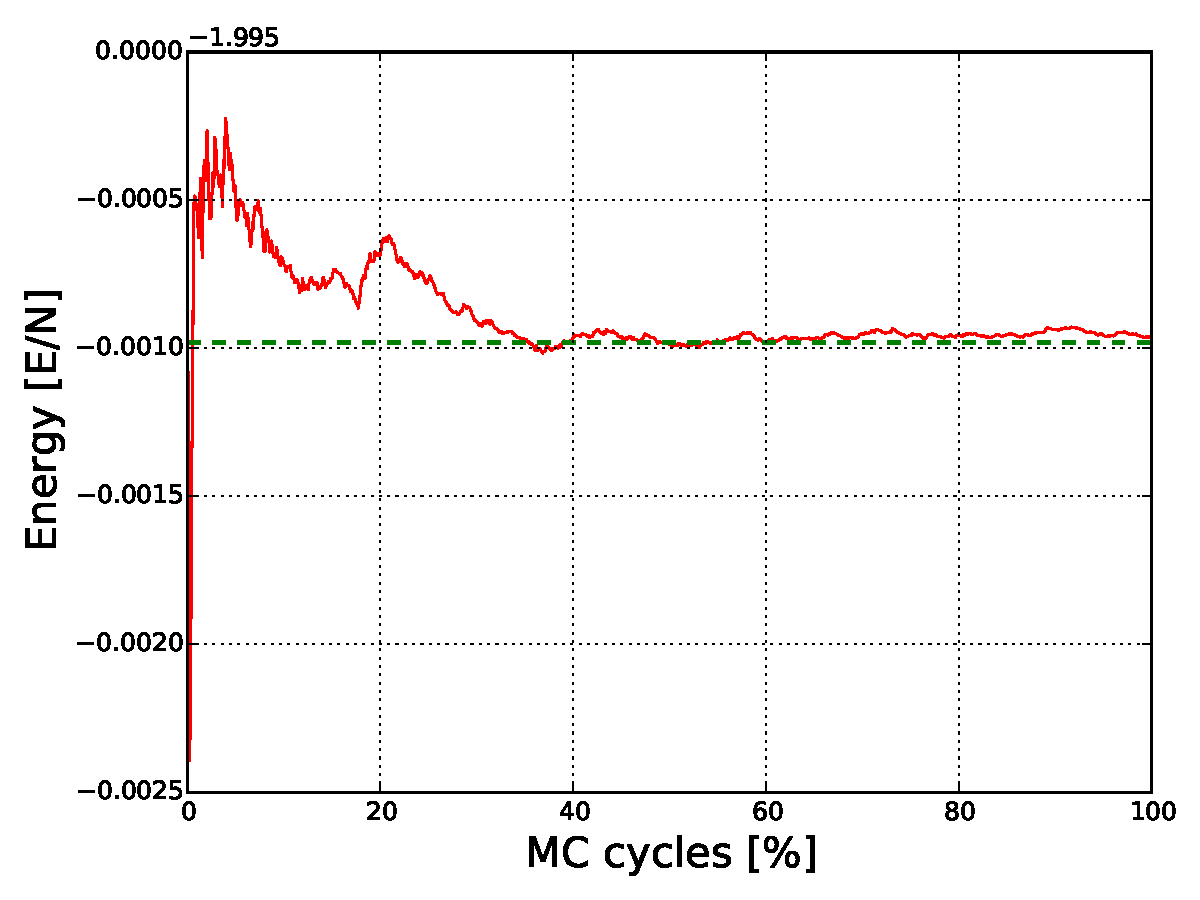
\includegraphics[width=\linewidth]{result/bilder/2x2/energy22}
        \caption{}
    \end{subfigure}%
    ~ 
    \begin{subfigure}{0.5\textwidth}
    	\centering
    	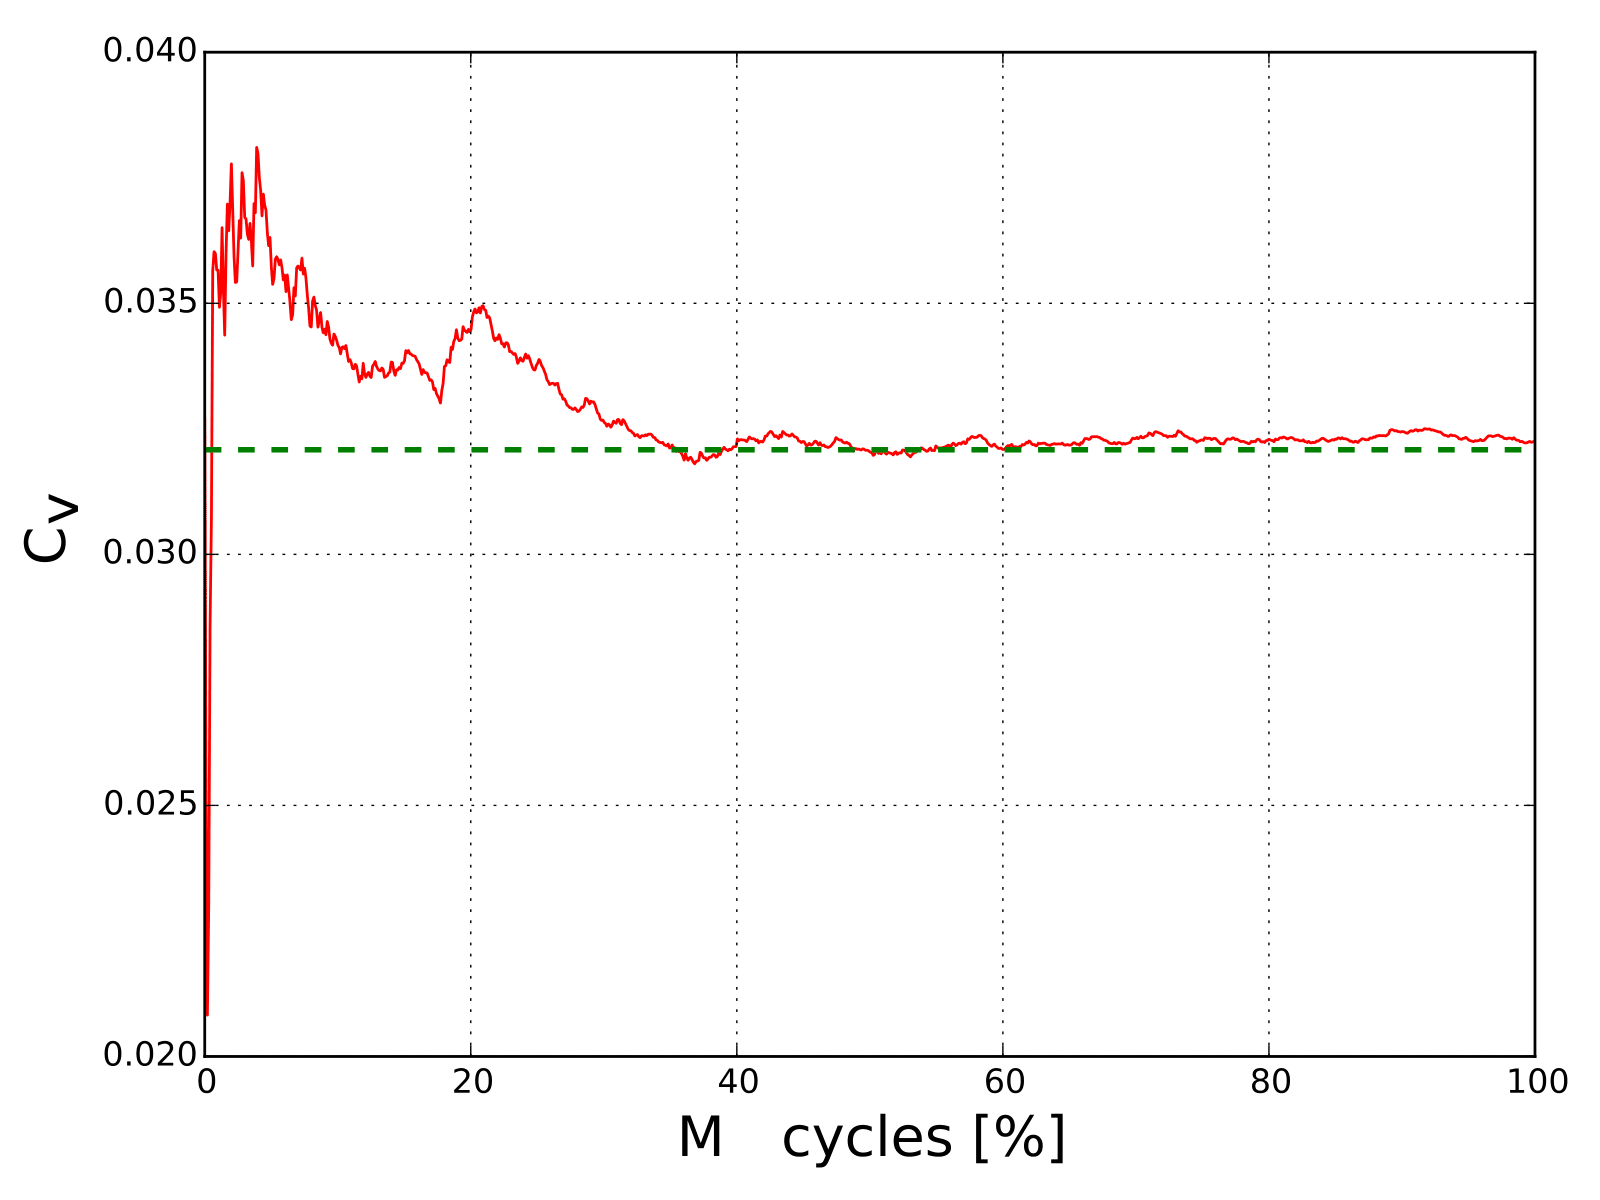
\includegraphics[width=\linewidth]{result/bilder/2x2/cv22_}
    	\caption{}
    \end{subfigure}
    \begin{subfigure}{0.5\textwidth}
        \centering
        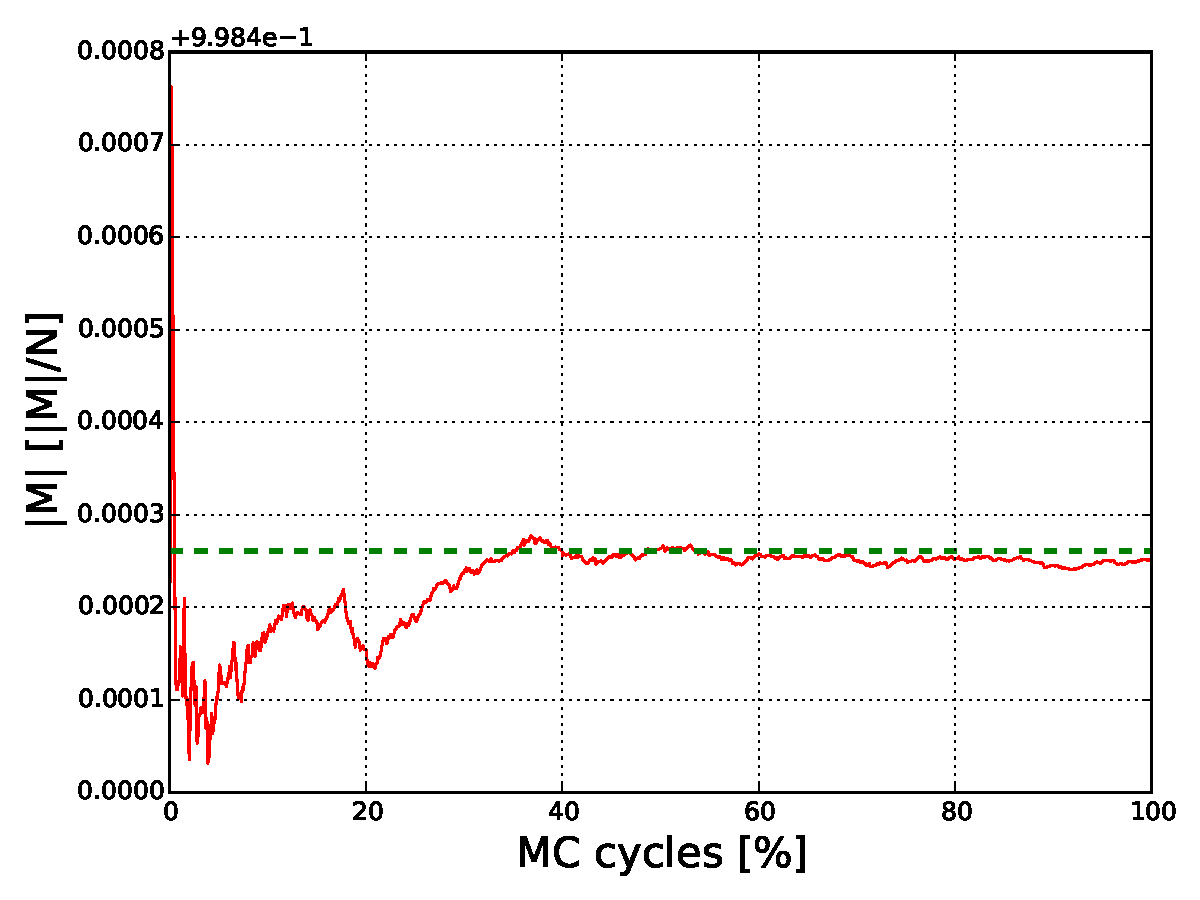
\includegraphics[width=\linewidth]{result/bilder/2x2/mabs22}
        \caption{}
    \end{subfigure}%
    ~ 
    \begin{subfigure}{0.5\textwidth}
        \centering
        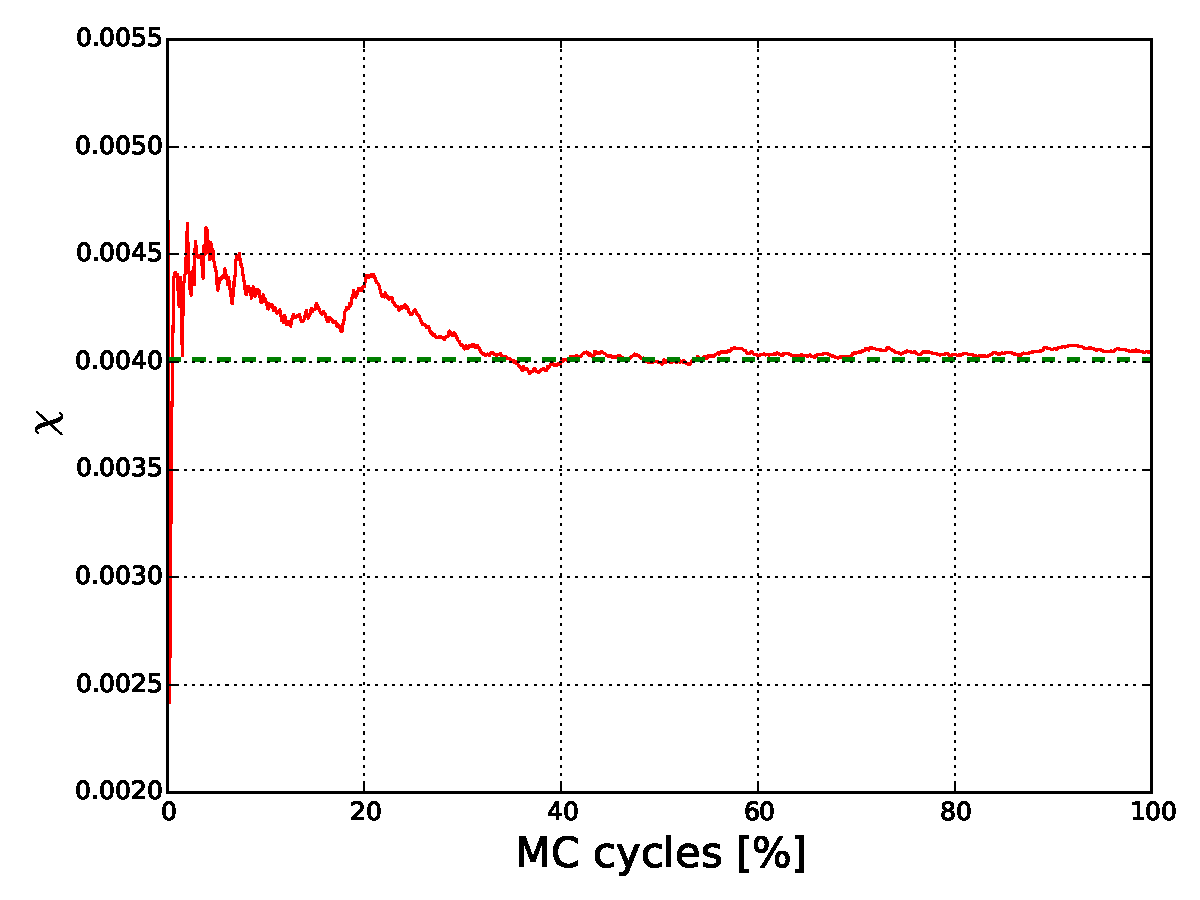
\includegraphics[width=\linewidth]{result/bilder/2x2/chi22}
        \caption{}
    \end{subfigure}
    \caption{a) Subplots shows how the expectation value for the different values varies, plotted with the number of Monte Carlo cycles on the x-axis.}
    \label{22results}
\end{figure}


As one can see from the graphs above the values tends quicly towards the numerically found expectation value. Below is a plot showing the difference between the numerical and analytical solutions. This will just be a rescaling of the plots. From these plots it is a good approximation when the Monte Carlo simulation has done about $40\%$ of the cycles. At this point there is almost no difference between the numerical and analytical solutions.


\begin{figure}[H]
	\centering
	\begin{subfigure}{0.5\textwidth}
		\centering
		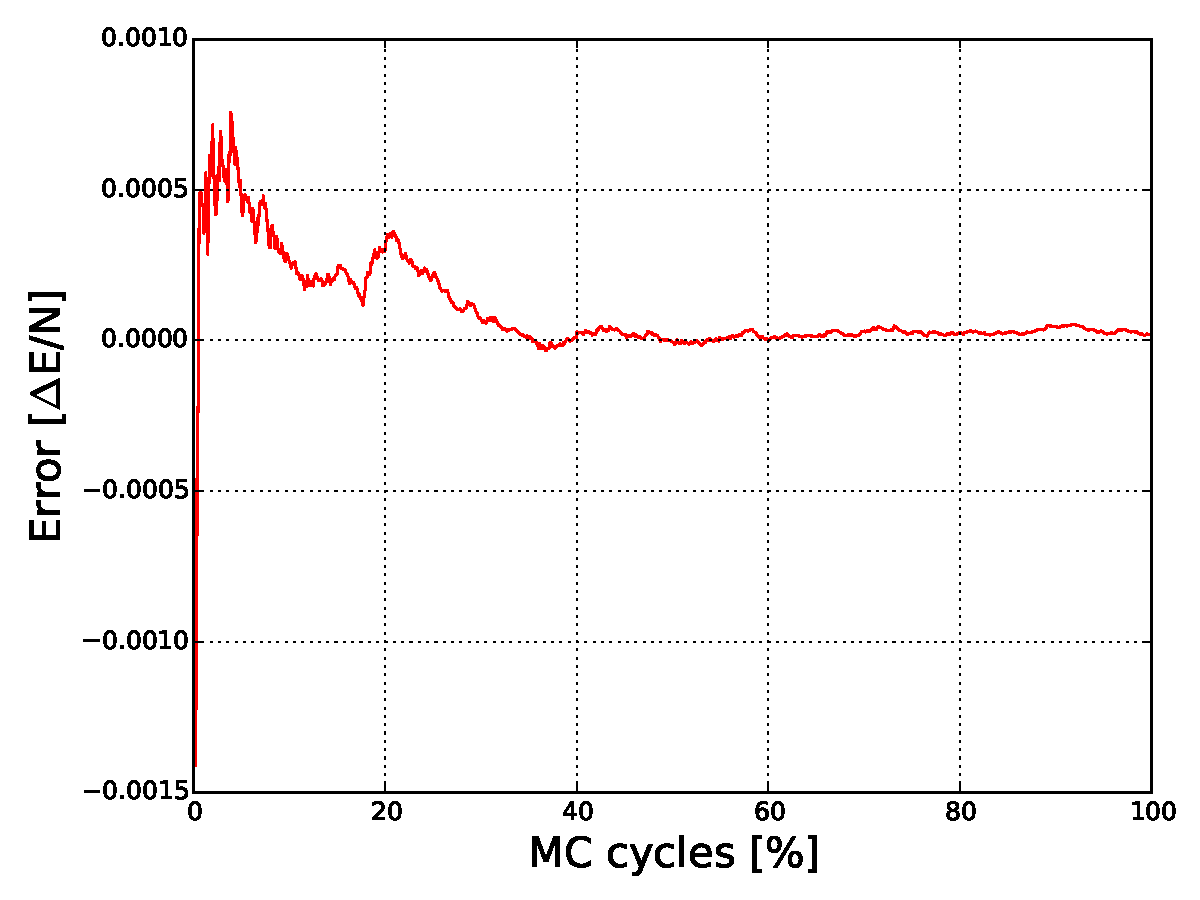
\includegraphics[width=\linewidth]{result/bilder/2x2/energyerror22}
		\caption{}
	\end{subfigure}%
	~ 
	\begin{subfigure}{0.5\textwidth}
		\centering
		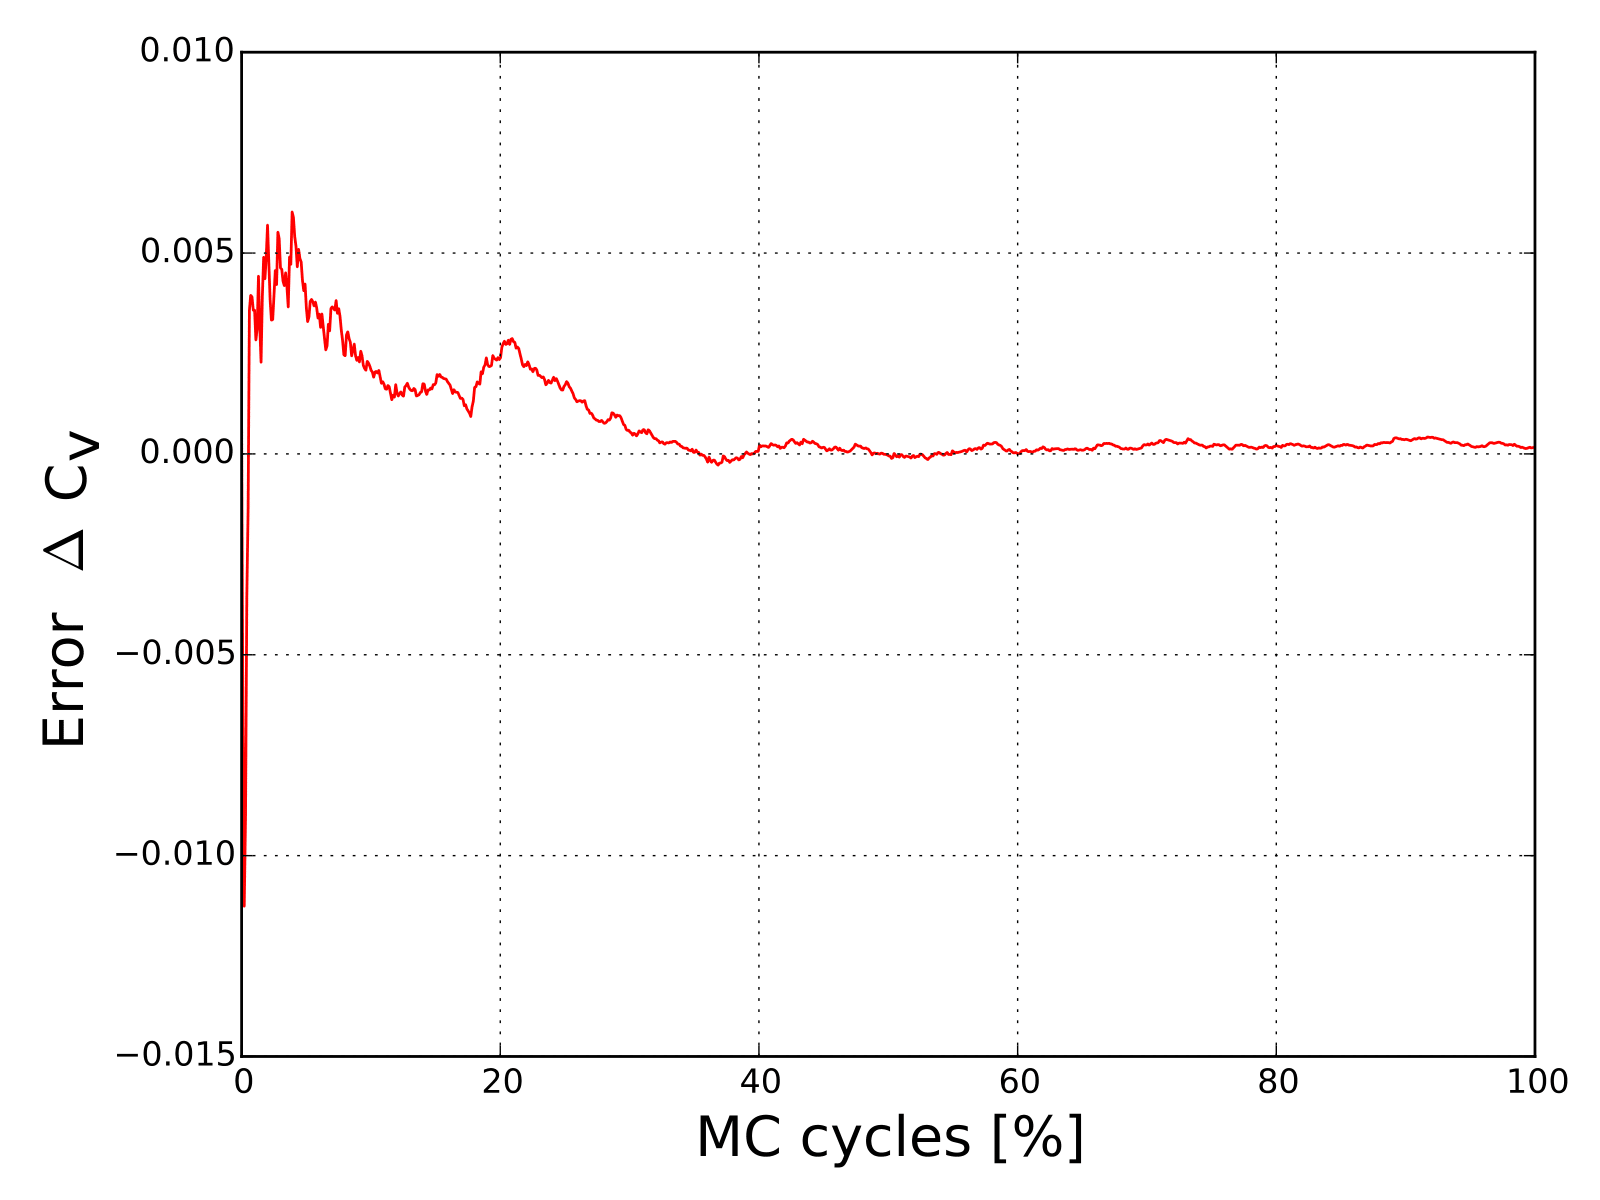
\includegraphics[width=\linewidth]{result/bilder/2x2/cverror22_}
		\caption{}
	\end{subfigure}
	\begin{subfigure}{0.5\textwidth}
		\centering
		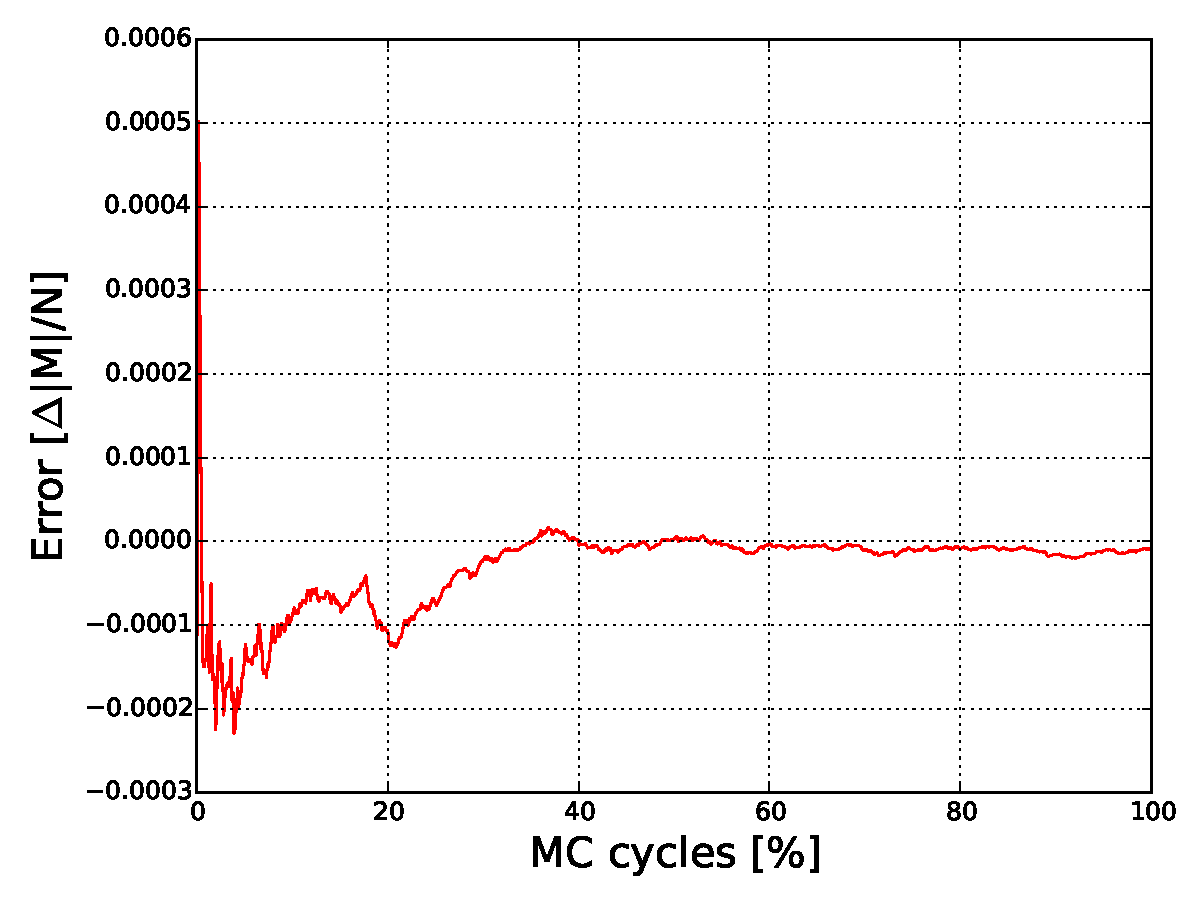
\includegraphics[width=\linewidth]{result/bilder/2x2/mabserror22}
		\caption{}
	\end{subfigure}%
	~ 
	\begin{subfigure}{0.5\textwidth}
		\centering
		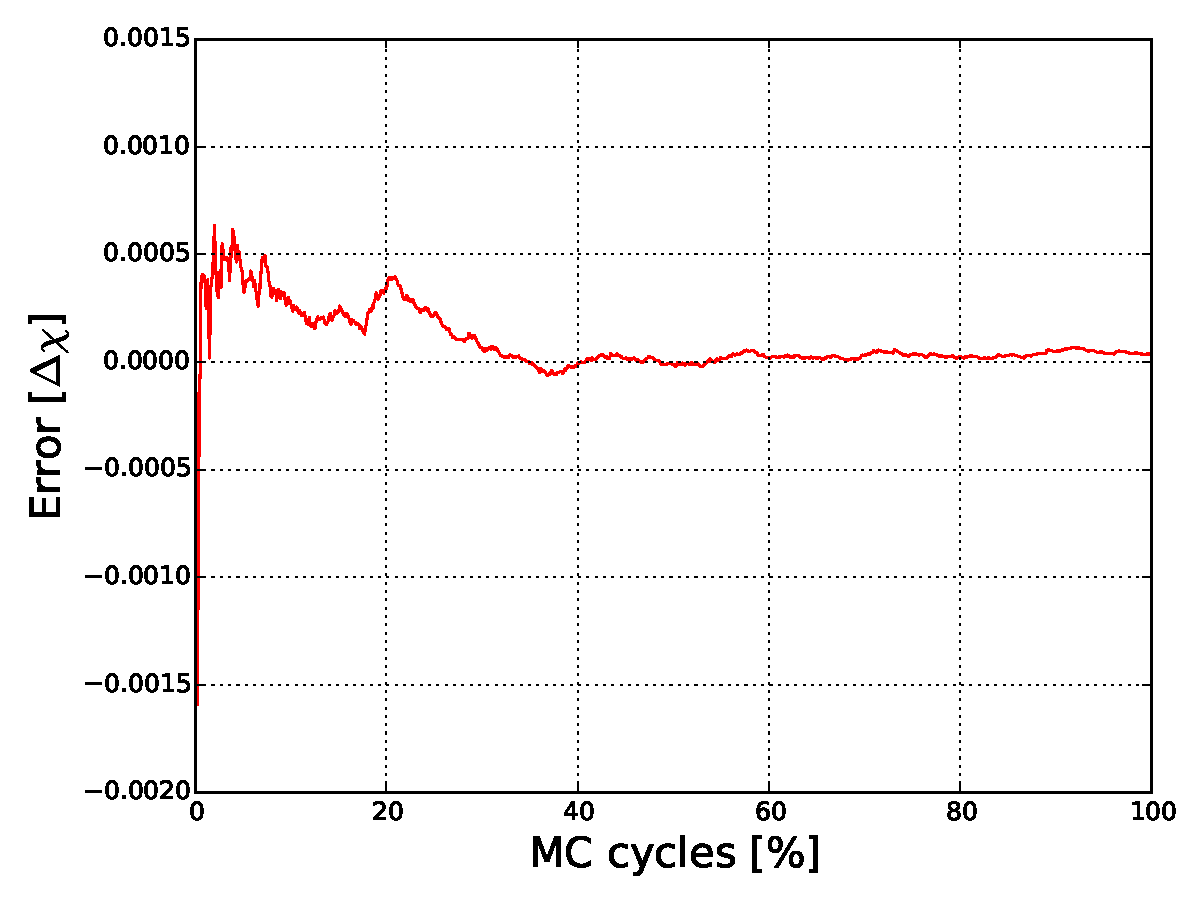
\includegraphics[width=\linewidth]{result/bilder/2x2/chierror22}
		\caption{}
	\end{subfigure}
	\caption{a) Shows how the the error develops for all the different expectation values.}
	\label{22error}
\end{figure}








\subsection{Numerical 20x20}

At this point no analytical solution is found, so from here on only the numerical solution is studied. All plots were made with $10*10^6$ cycles. For the $20\times20$ grid who different starting points where analyzed. On the right side a plot with random spin configuration in initialized. While on the left hand side the system is initialized with all spins in the same direction. Firstly the energy and magnetic moment is analyzed for $T=1$. Then a higher temperature state is analyzed with $T=2.4$

\begin{figure}[H]
    \centering
    \begin{subfigure}{0.5\textwidth}
        \centering
        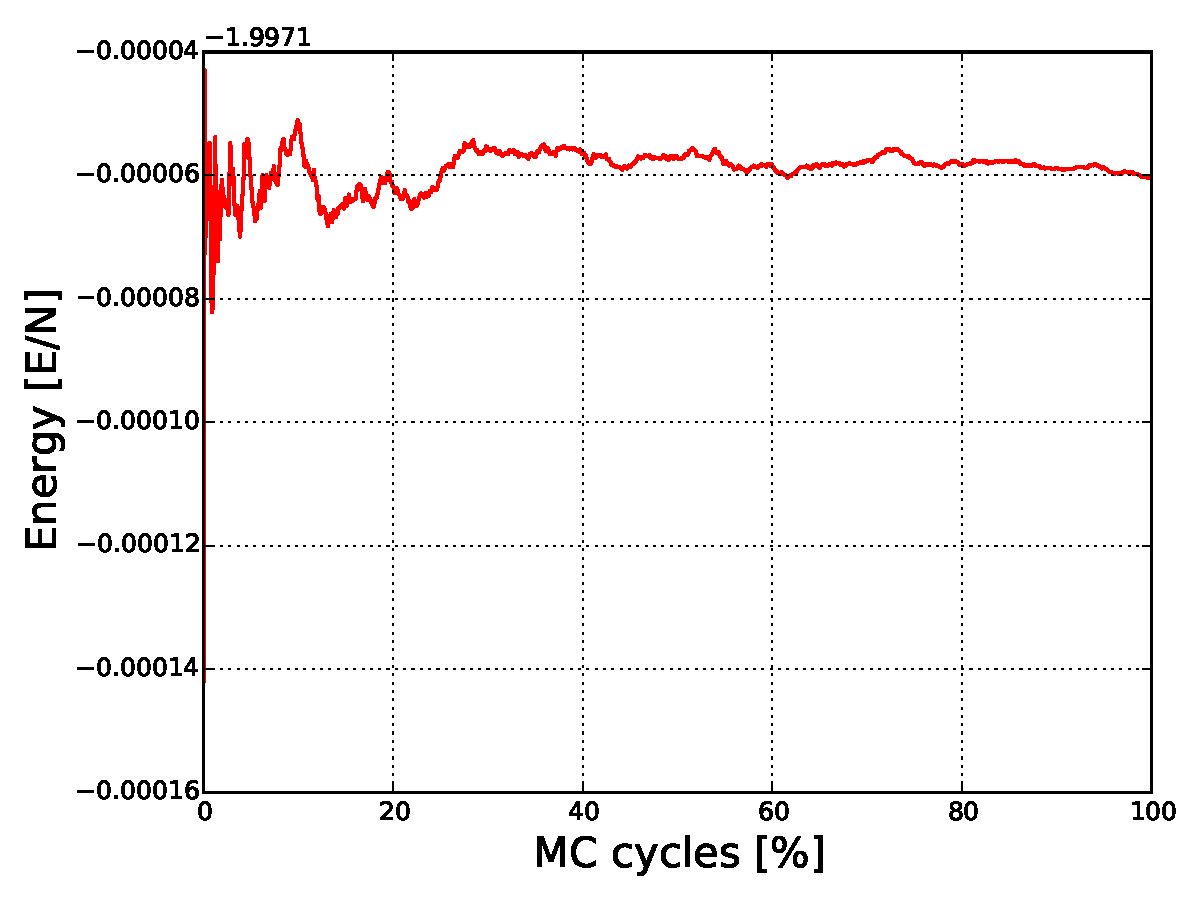
\includegraphics[width=\linewidth]{result/bilder/20x20/E-N20-T1}
        \caption{}
    \end{subfigure}%
    ~ 
    \begin{subfigure}{0.5\textwidth}
        \centering
        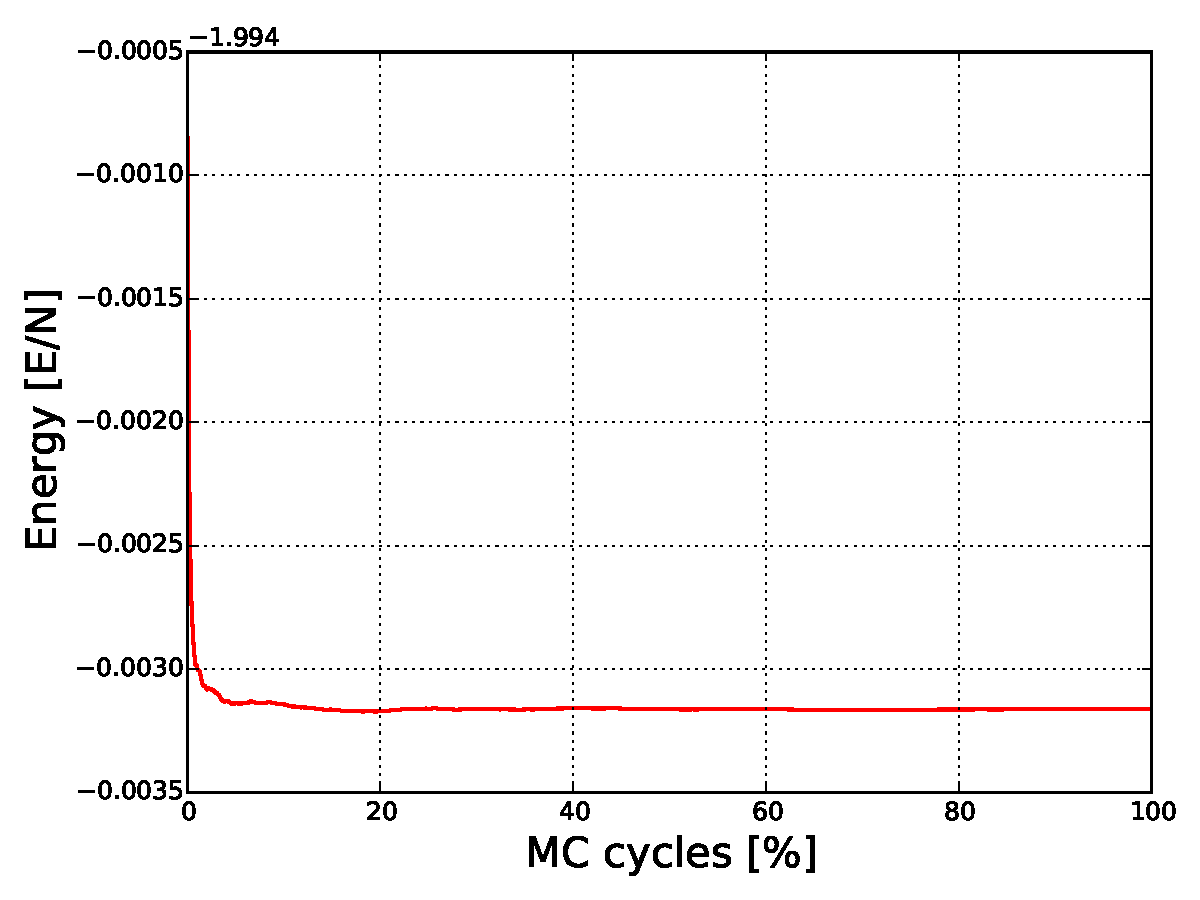
\includegraphics[width=\linewidth]{result/bilder/20x20/E-N20-T1-RNG}
        \caption{}
    \end{subfigure}
    \caption{The figure shows the development of the energy. In the program $T$ is sat to $1$. }
    \label{fig:}
\end{figure}

\begin{figure}[H]
    \centering
    \begin{subfigure}{0.5\textwidth}
        \centering
        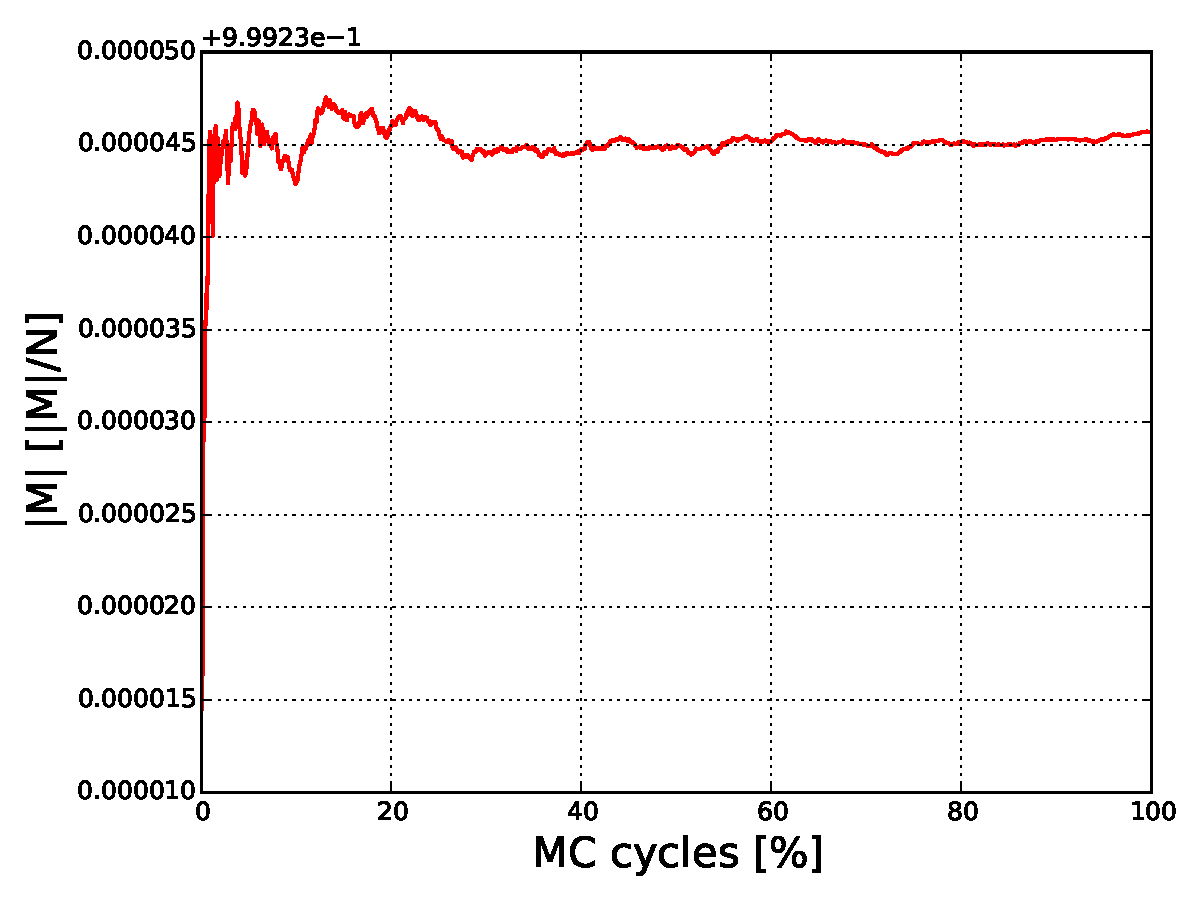
\includegraphics[width=\linewidth]{result/bilder/20x20/M-N20-T1}
        \caption{}
    \end{subfigure}%
    ~ 
    \begin{subfigure}{0.5\textwidth}
        \centering
        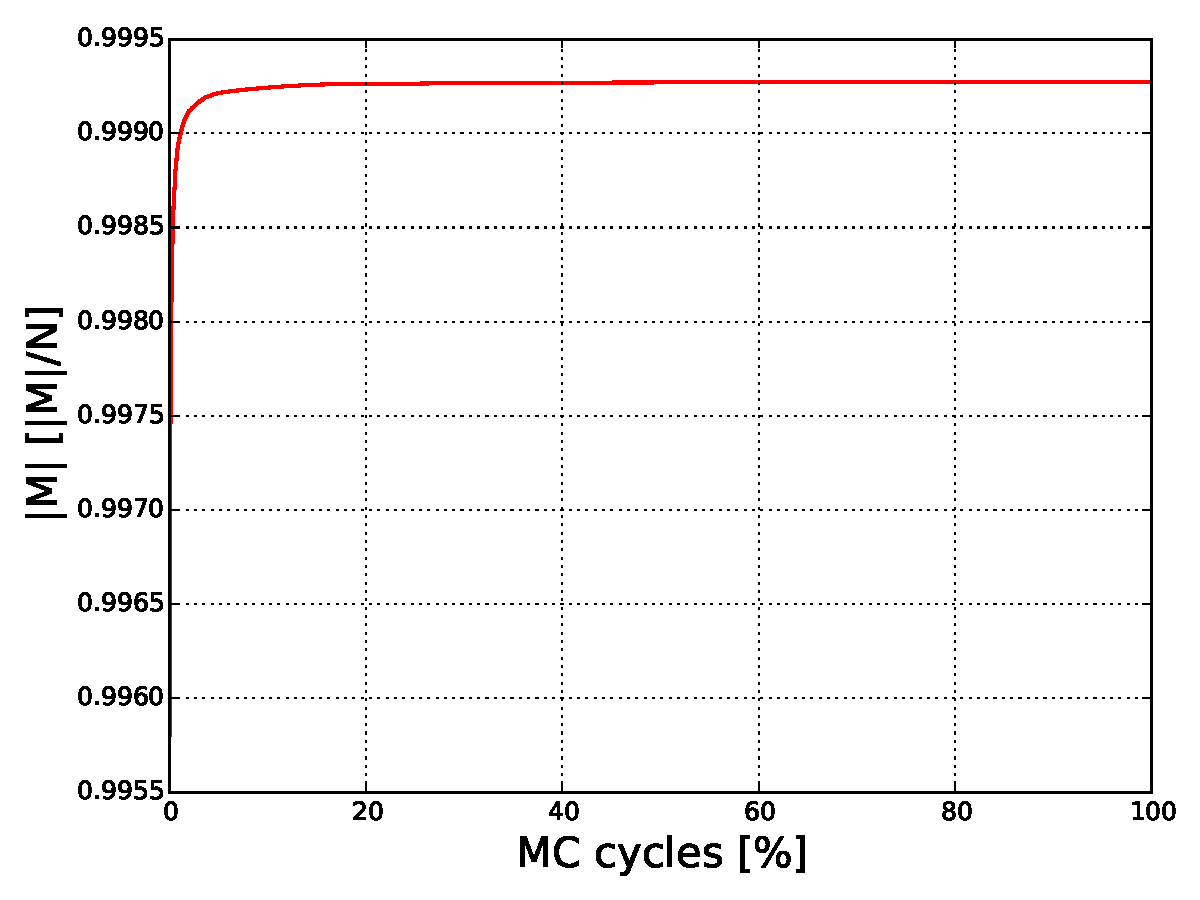
\includegraphics[width=\linewidth]{result/bilder/20x20/M-N20-T1-RNG}
        \caption{}
    \end{subfigure}
    \caption{The figure shows the development of the Magnetic moment. In the program $T$ is sat to $1$. }
    \label{fig:}
\end{figure}

A clear trend is visible for the initialized ordered case. This has more irregularities and uses longer time to reach equilibrium. This is because it started out ordered in a manner that was not energetically beneficial for the system. Whereas the random initialized case has a much smoother curve due to it starting in a more energetically favored position. For the next plots the temperature was increased, to look at the effects temperature has on the system.




\begin{figure}[H]
    \centering
    \begin{subfigure}{0.5\textwidth}
        \centering
        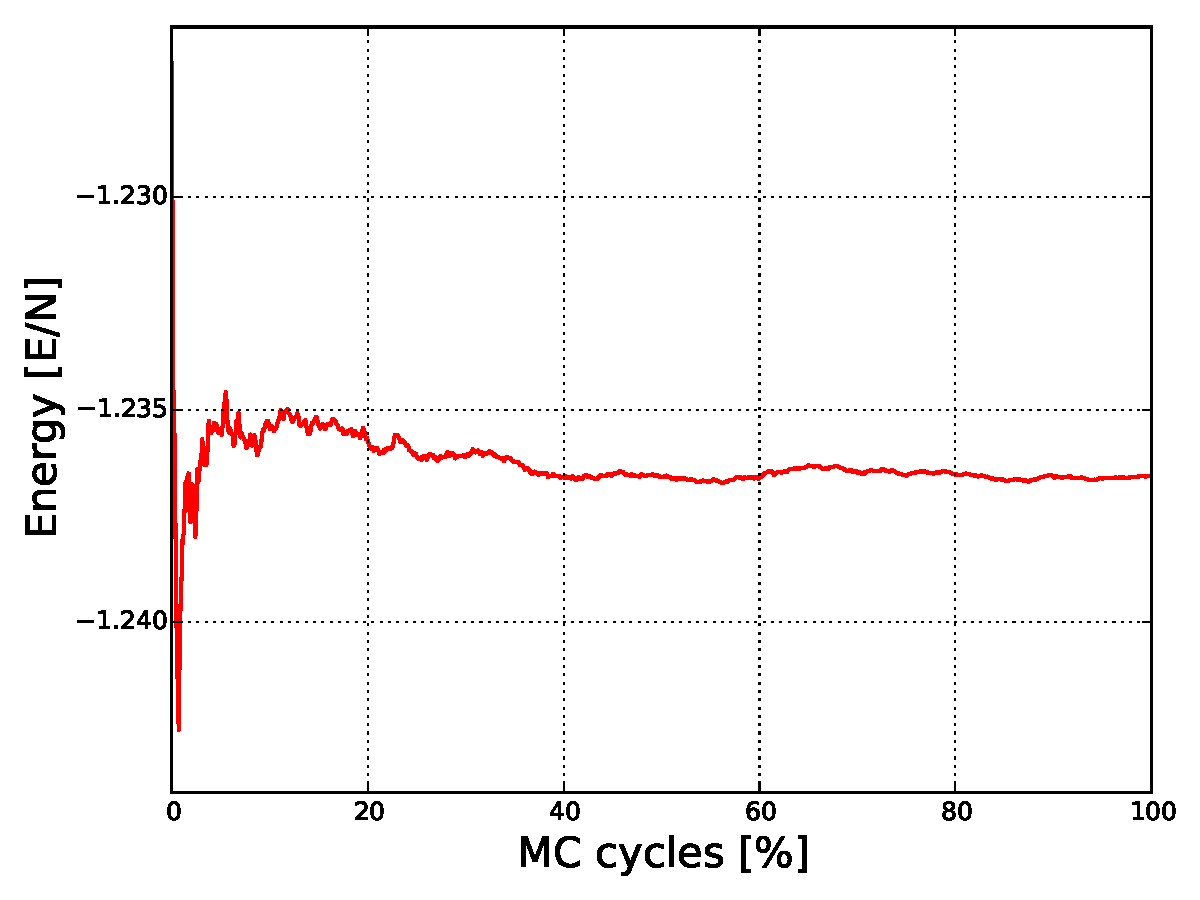
\includegraphics[width=\linewidth]{result/bilder/20x20/E-N20-T24}
        \caption{}
    \end{subfigure}%
    ~ 
    \begin{subfigure}{0.5\textwidth}
        \centering
        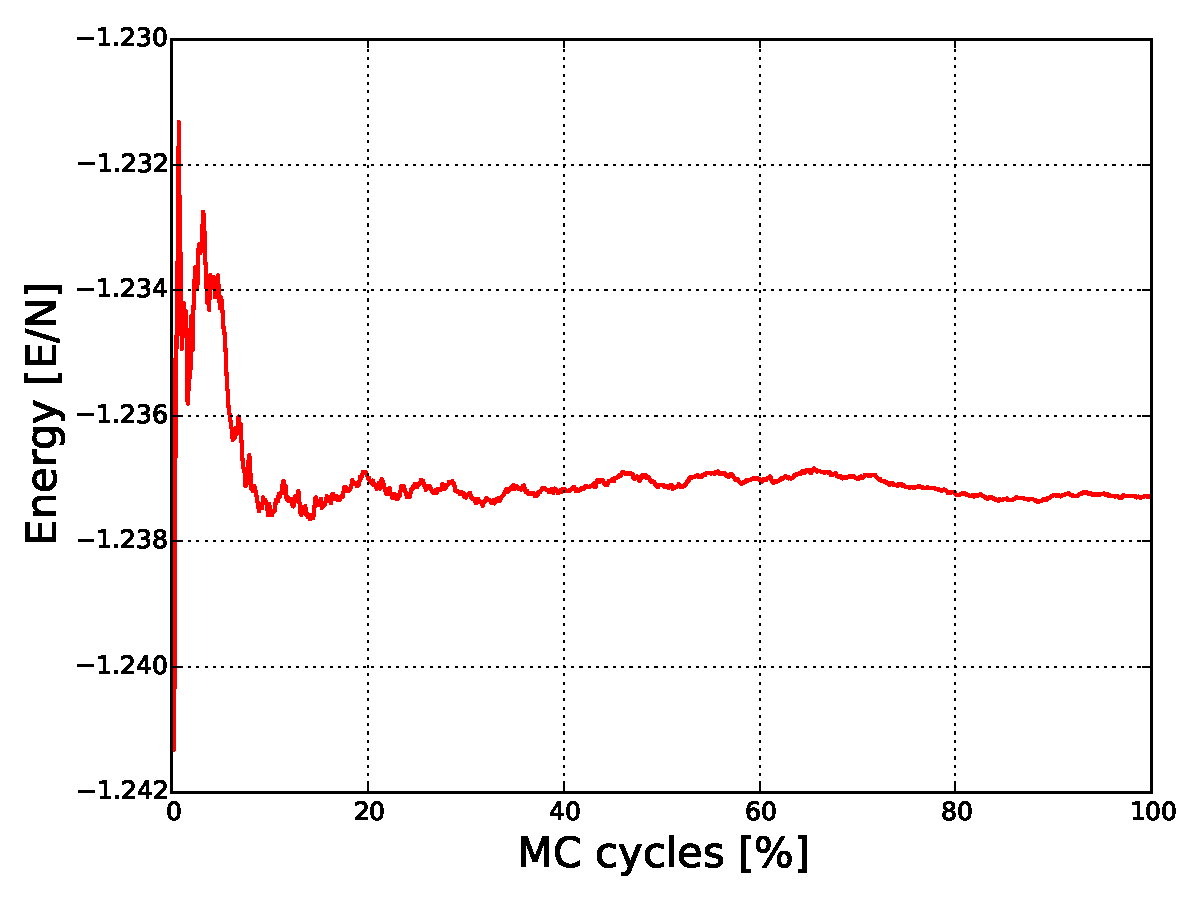
\includegraphics[width=\linewidth]{result/bilder/20x20/E-N20-T24-RNG}
        \caption{}
    \end{subfigure}
    \caption{The figure shows the development of the energy. In the program $T$ is sat to $2.4$.}
    \label{fig:}
\end{figure}

\begin{figure}[H]
    \centering
    \begin{subfigure}{0.5\textwidth}
        \centering
        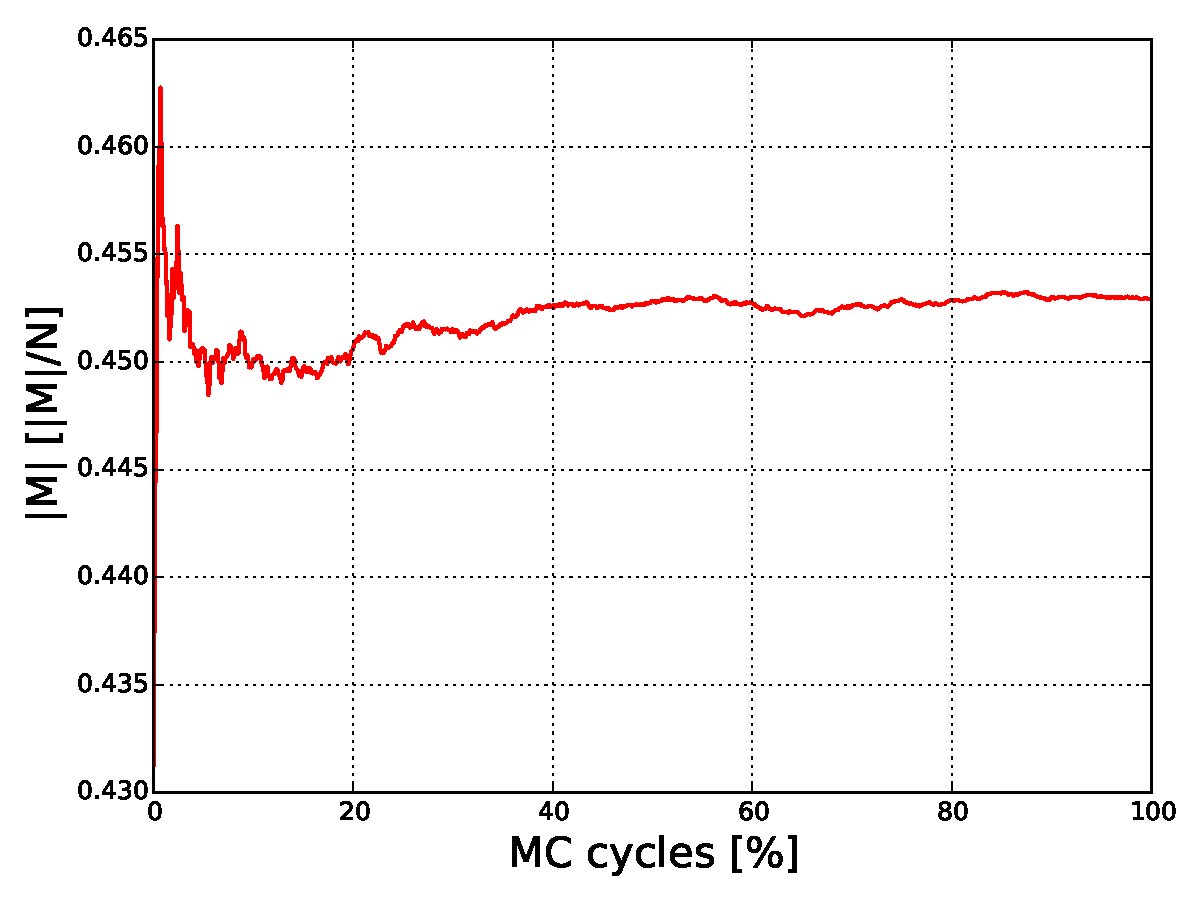
\includegraphics[width=\linewidth]{result/bilder/20x20/M-N20-T24}
        \caption{}
    \end{subfigure}%
    ~ 
    \begin{subfigure}{0.5\textwidth}
        \centering
        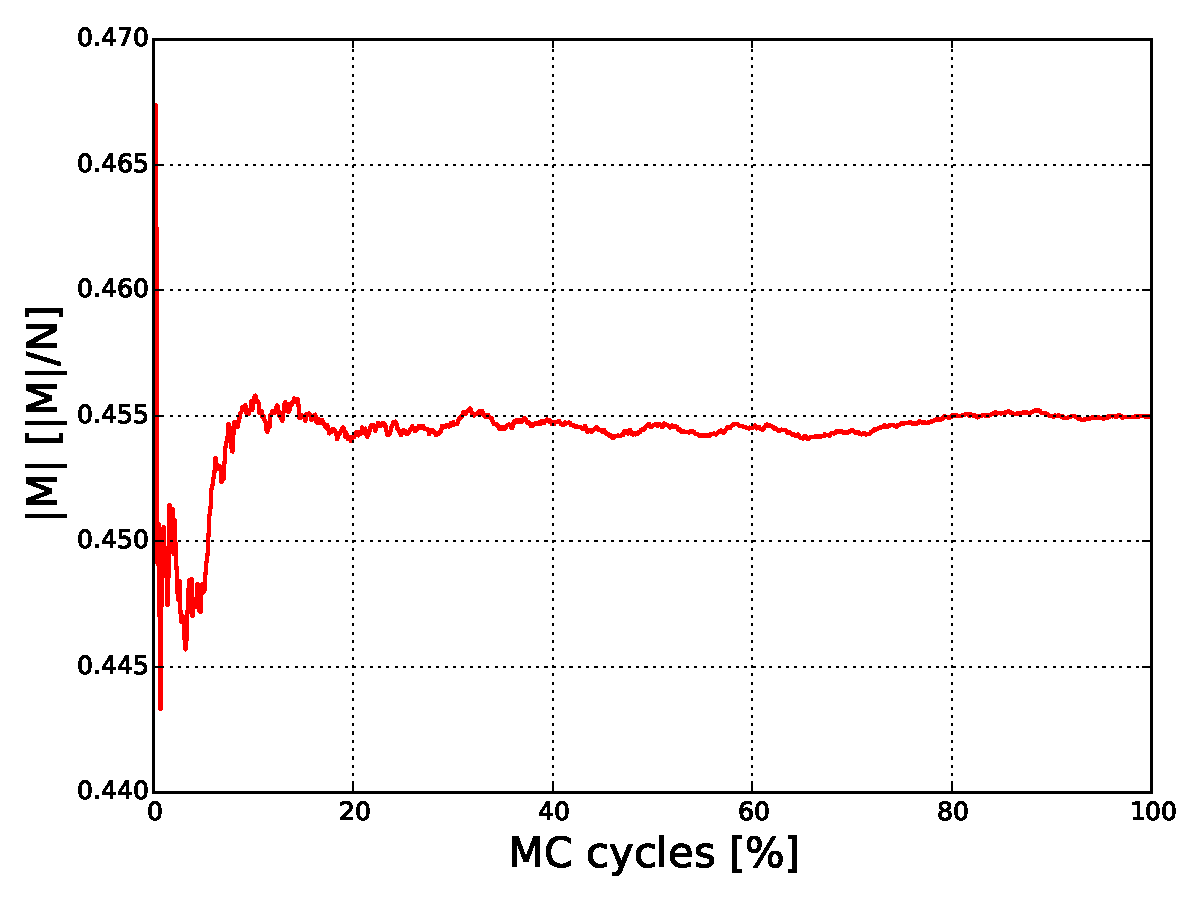
\includegraphics[width=\linewidth]{result/bilder/20x20/M-N20-T24-RNG}
        \caption{}
    \end{subfigure}
    \caption{The figure shows the development of the Magnetic moment. In the program $T$ is sat to $2.4$.}
    \label{fig:}
\end{figure}

For the higher temperature the Helmholtz free energy equations temperature term becomes more impactull. $F=E-TS$. This is visible in the random initialized version. This is now not so smooth and varies more. In all of these cases, for $T=1$ and $T=2.4$ the same variations in the first part of the cycles can be observed. The next plot hows what the plots for $T=1$ would have looked like if the first $10^5$ steps are not included.


\begin{figure}[H]
    \centering
    \begin{subfigure}{0.5\textwidth}
        \centering
        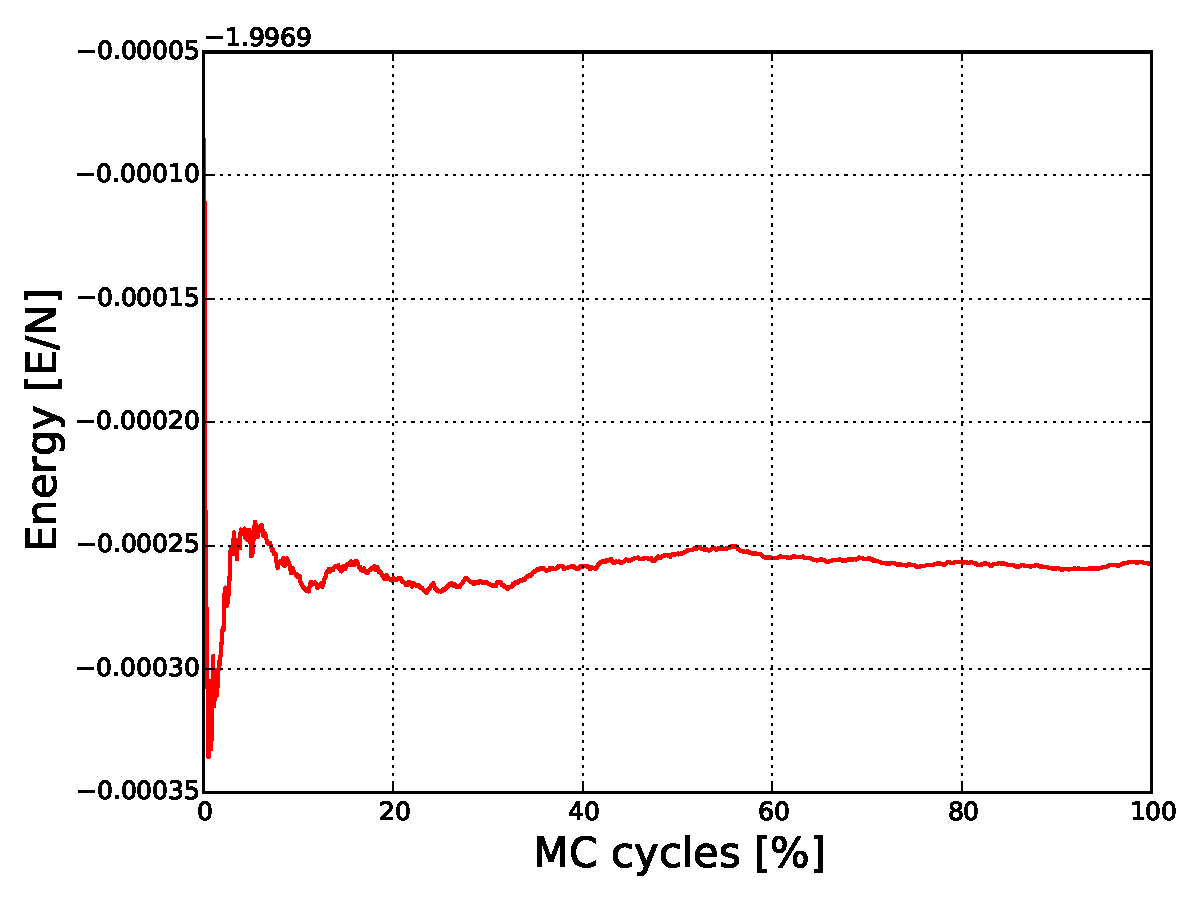
\includegraphics[width=\linewidth]{result/bilder/20x20/E-N20-T1-Term}
        \caption{}
    \end{subfigure}%
    ~ 
    \begin{subfigure}{0.5\textwidth}
        \centering
        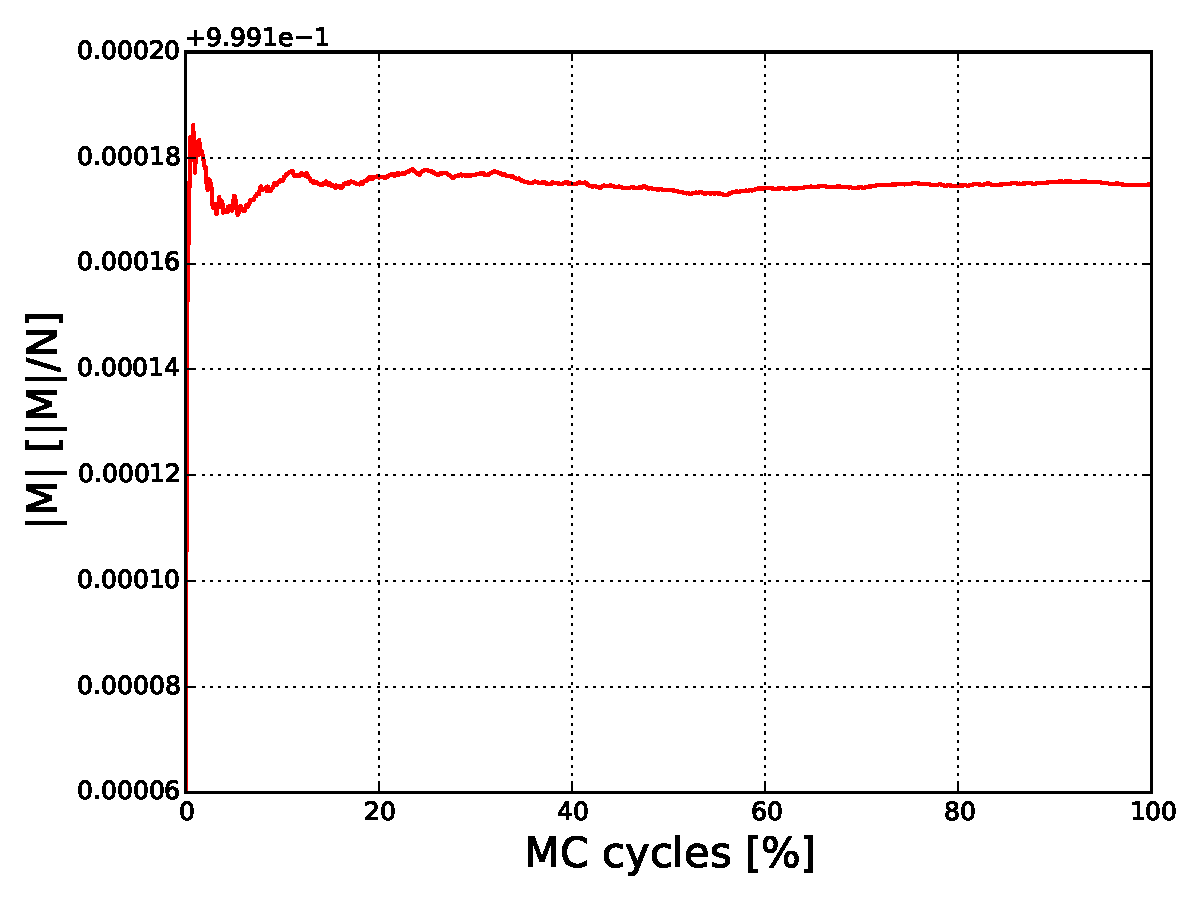
\includegraphics[width=\linewidth]{result/bilder/20x20/M-N20-T1-Term}
        \caption{}
    \end{subfigure}
    \caption{The development of energy when $T = 1$, excluding the first $10^5$ steps.  }
    \label{fig:equilibrium}
\end{figure}


For the remainder of the report $10^5$ Monte Carlo cycles will be used to obtain equilibrium. This is a value chosen because if more cycles were chosen this would require more computing power, if less cycles were chosen then the results would not give the approximate expectation value. 












\subsection{Accepted configurations}

In the previous section the differences between temperature and initial states were studied. In this section a study of the acceptance rate of flips is made, not focusing on the energy or magnetic moment of the system. As for the previous section, left figures shows a ordered initial configuration while the right hand side shows a random starting point.

\begin{figure}[H]
    \centering
    \begin{subfigure}{0.5\textwidth}
        \centering
        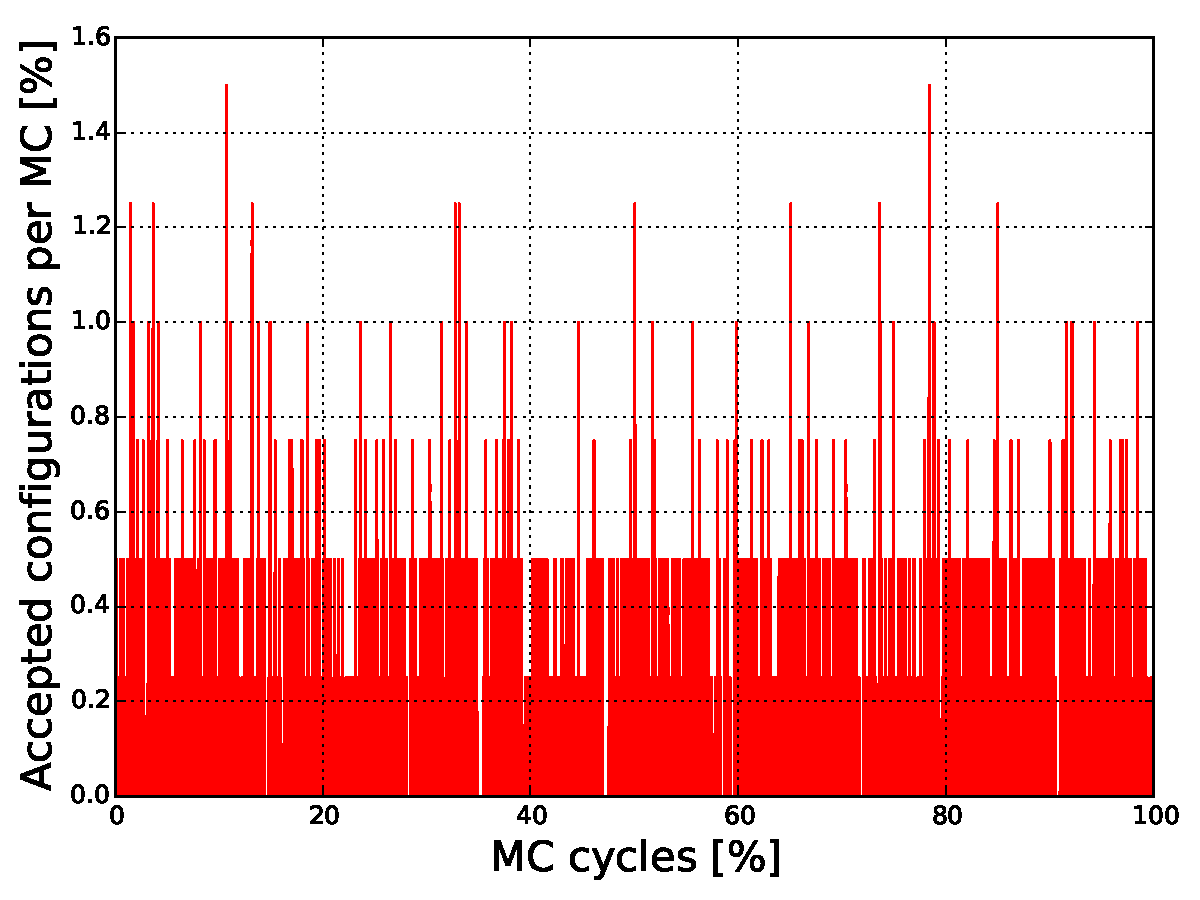
\includegraphics[width=\linewidth]{result/bilder/config/energy22-MC1000000T1-configN20}
        \caption{}
    \end{subfigure}%
    ~ 
    \begin{subfigure}{0.5\textwidth}
        \centering
        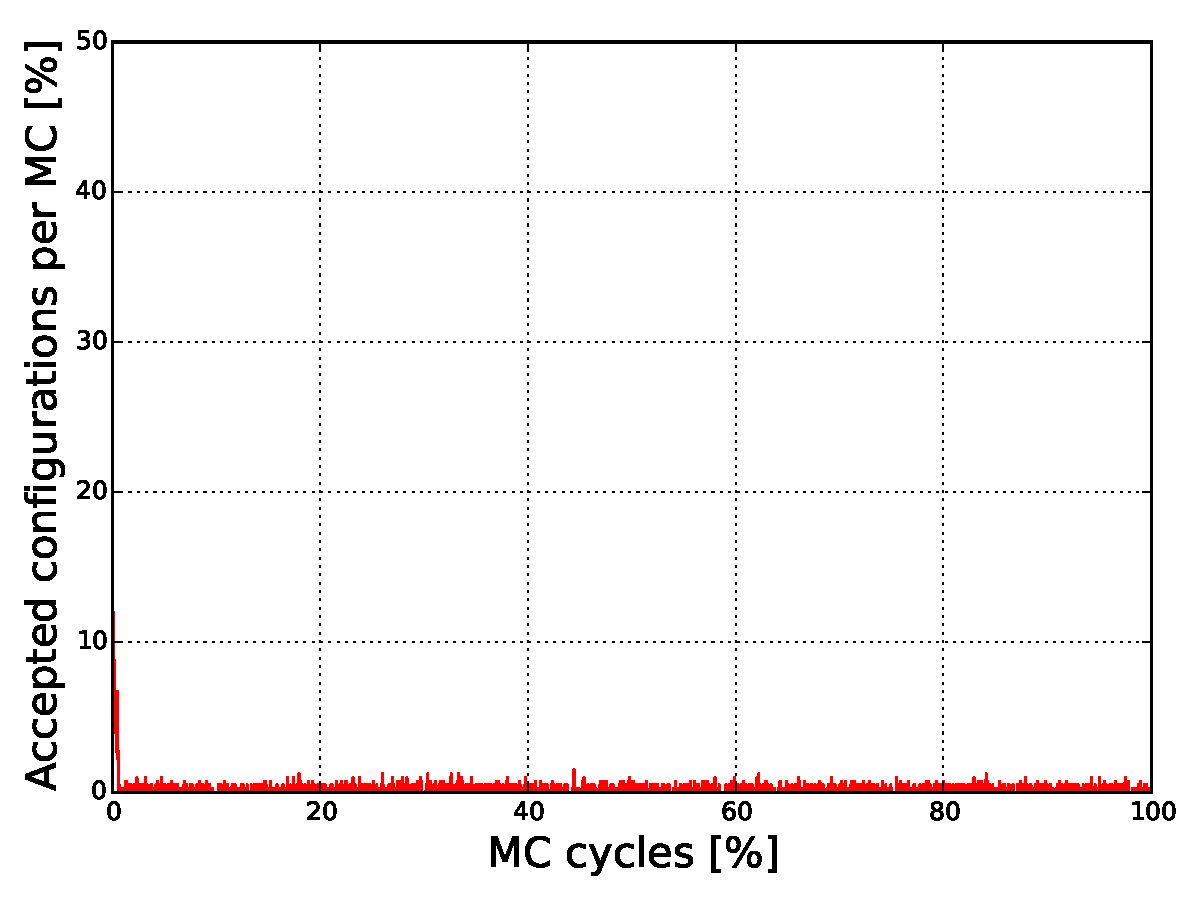
\includegraphics[width=\linewidth]{result/bilder/config/energy22-MC1000000T1-config-RNGN20}
        \caption{}
    \end{subfigure}
    \caption{Plot shows the acceptance rate of flipped spins at temperature one, with $10^6$ cycles. }
    \label{fig:config-T1}
\end{figure}
The right configuration seems to have a lower acceptance rate then the left one. This is due to the scaling and first steps. When looking at the y-axis one can see that for the right configuration acceptance is high. 

\begin{figure}[H]
    \centering
    \begin{subfigure}{0.5\textwidth}
        \centering
        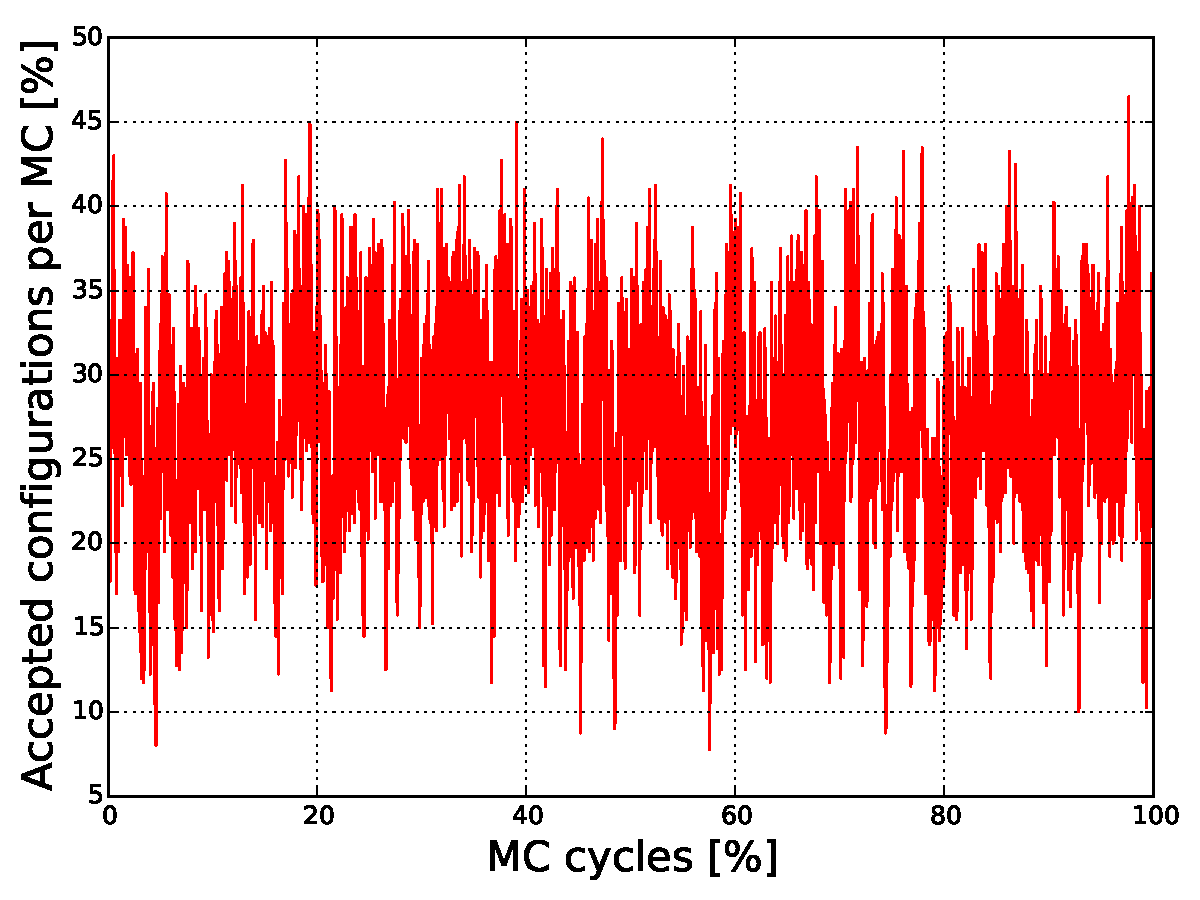
\includegraphics[width=\linewidth]{result/bilder/config/energy22-MC1000000T24-configN20}
        \caption{}
    \end{subfigure}%
    ~ 
    \begin{subfigure}{0.5\textwidth}
        \centering
        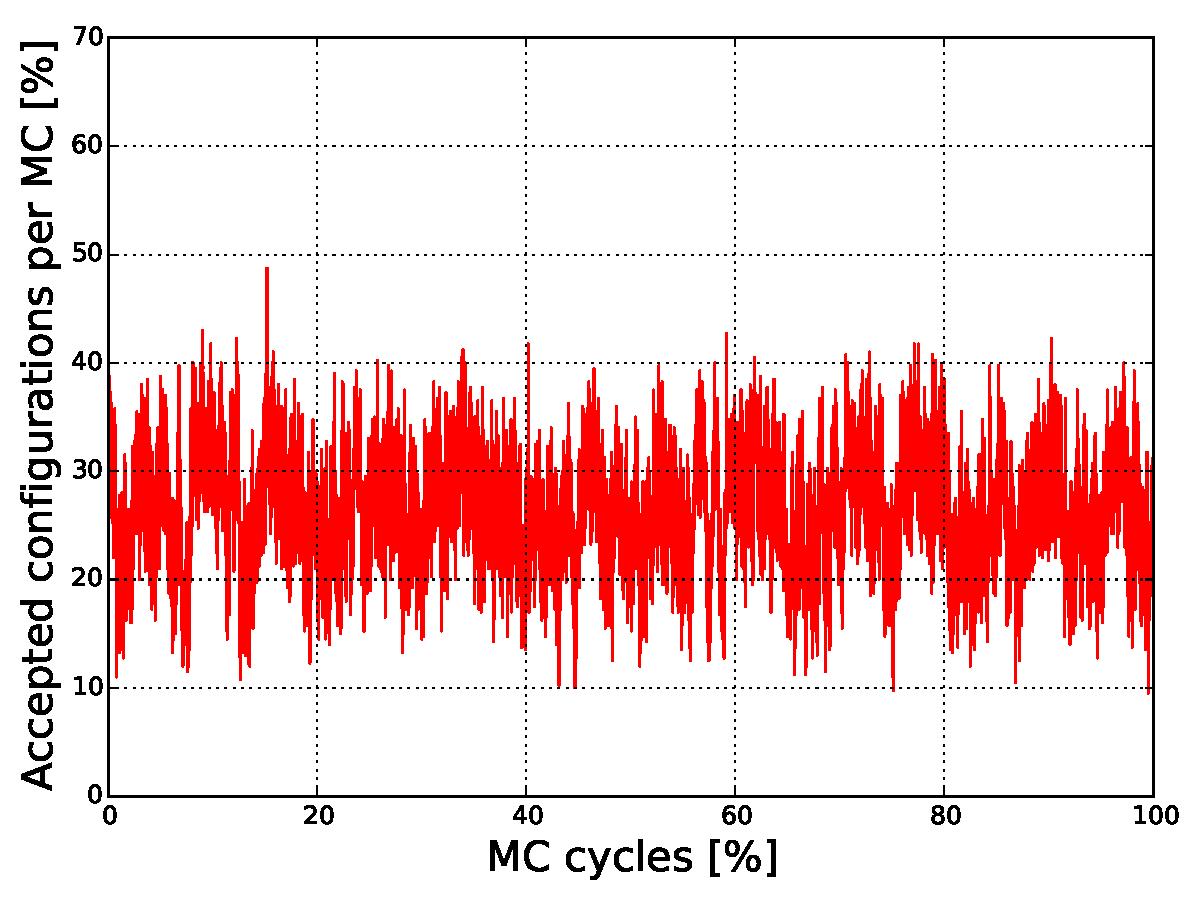
\includegraphics[width=\linewidth]{result/bilder/config/energy22-MC1000000T24-config-RNGN20}
        \caption{}
    \end{subfigure}
    \caption{Plot shows the acceptance rate of flipped spins at temperature $2.4$, with $10^6$ cycles. }
    \label{fig:config-T24}
\end{figure}

When comparing the two different temperatures the change in acceptance rate is noticeable. For higher temperatures the acceptance rate becomes over a factor of ten larger. 


\subsection{Probability distribution}

The probability distribution of energies for the two different temperatures are extreme.

\begin{figure}[H]
    \centering
    \begin{subfigure}{0.5\textwidth}
        \centering
        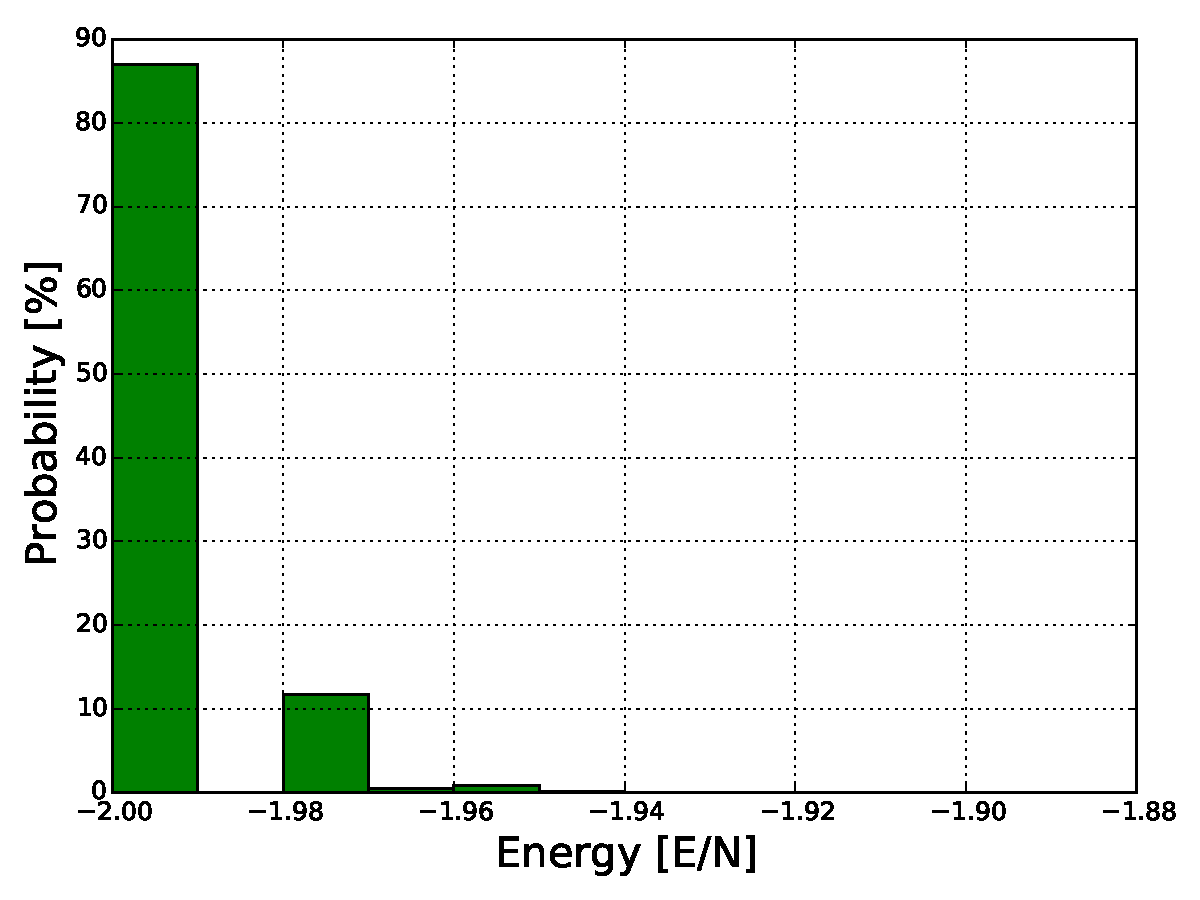
\includegraphics[width=\linewidth]{result/bilder/hist/MC1000000T1-distN20-hist}
        \caption{}
    \end{subfigure}%
    ~ 
    \begin{subfigure}{0.5\textwidth}
        \centering
        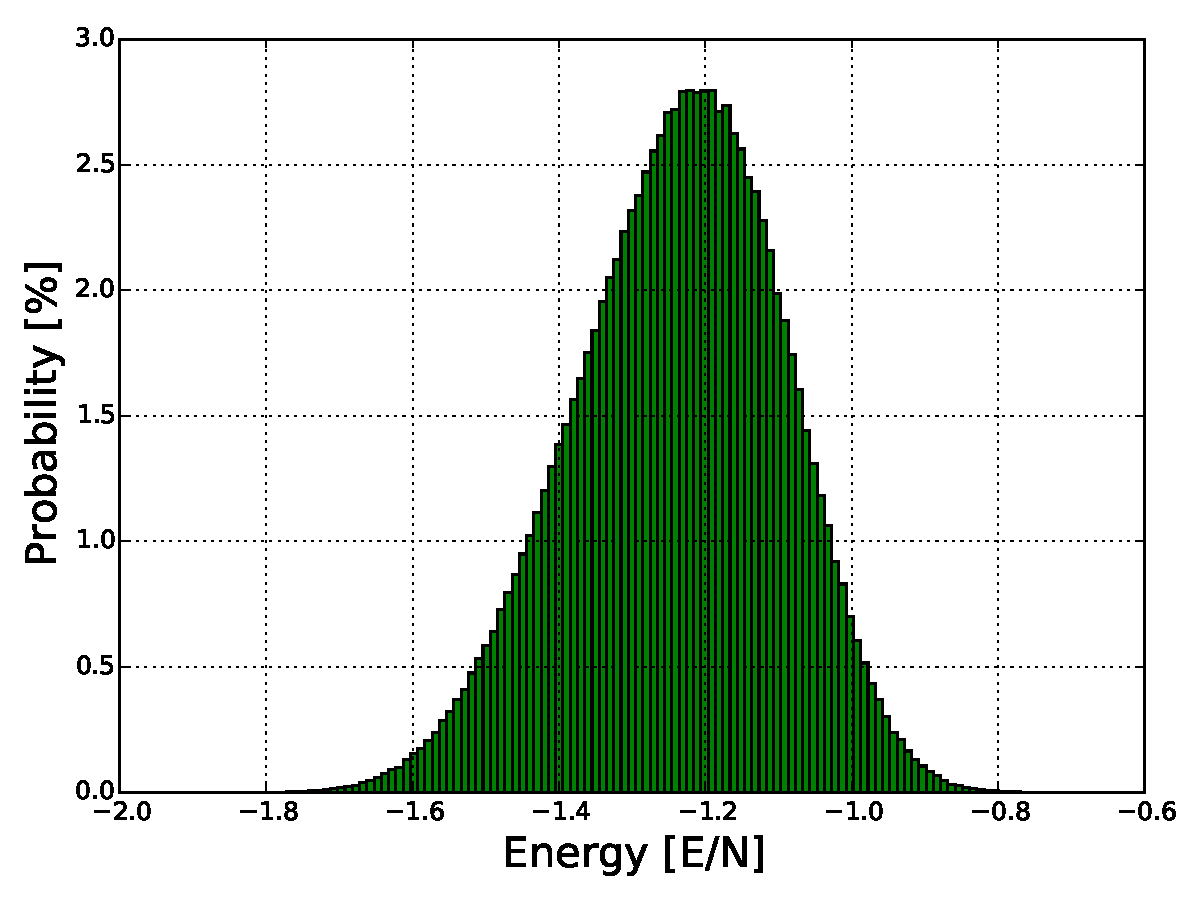
\includegraphics[width=\linewidth]{result/bilder/hist/MC1000000T24-distN20-hist}
        \caption{}
    \end{subfigure}
    \caption{The two figures shows the distribution of energy states at different temperatures. The left plot shows the distribution at temperature $1$ and the right plot shows the distribution at temperature $2.4$.}
    \label{fig:tc-chi-cv}
\end{figure}

The differences in distribution is due to the Boltzmann distribution used in the model. For the lowest temperature more states are expected to have the lower energy, while for the system with higher energy the distribution is expected to have a better distribution of energies. This also fits the results from the previous section well. For higher temperatures the system accepts more changes and the peak becomes broader. While for the low temperature few changes were accepted leading to a lower degree peak broadening.




















\subsection{Phase transition}

To study the phase transitions of the system several runs were done varying $L$ between $20-200$. The figures below shows a selection of the runs.


\begin{figure}[H]
    \centering
    \begin{subfigure}{0.5\textwidth}
        \centering
        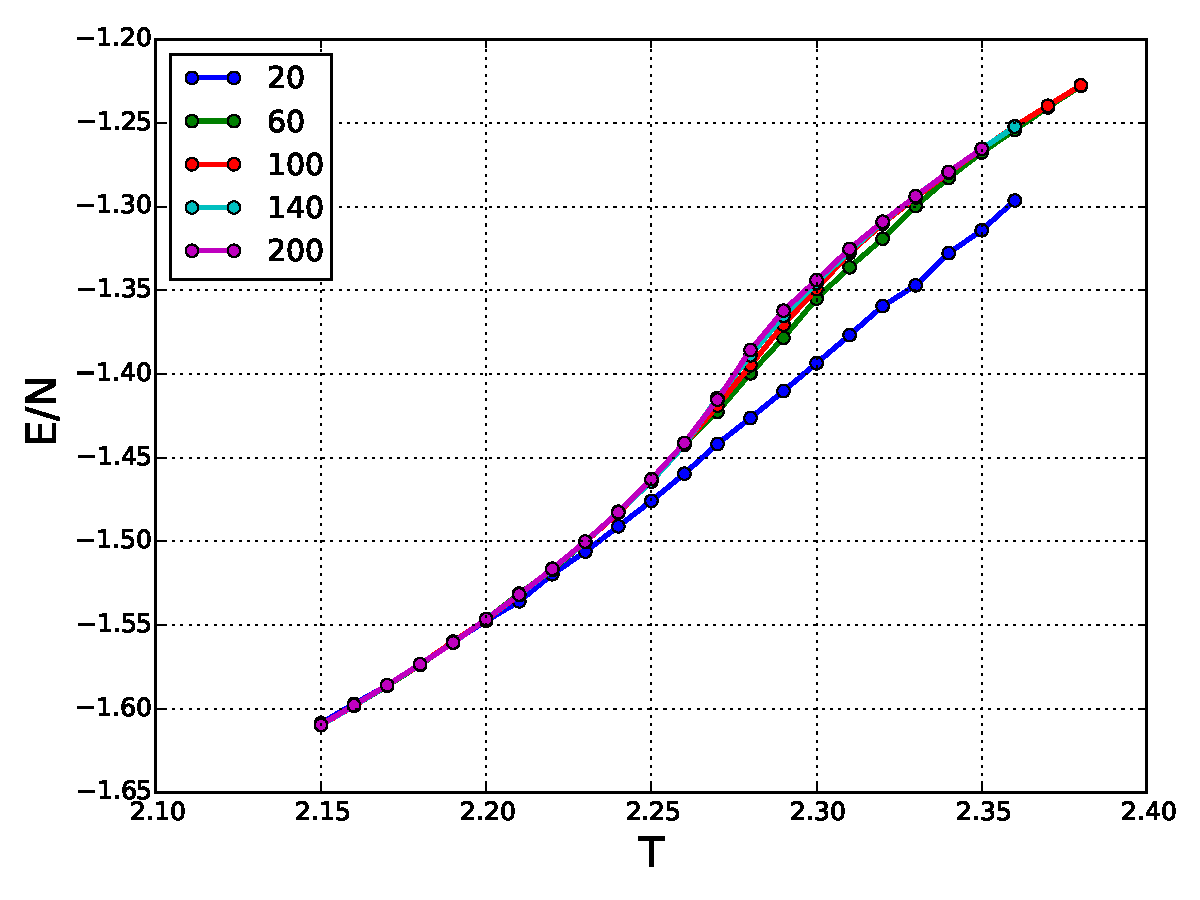
\includegraphics[width=\linewidth]{result/bilder/Tc/e-Tc}
        \caption{}
    \end{subfigure}%
    ~ 
    \begin{subfigure}{0.5\textwidth}
        \centering
        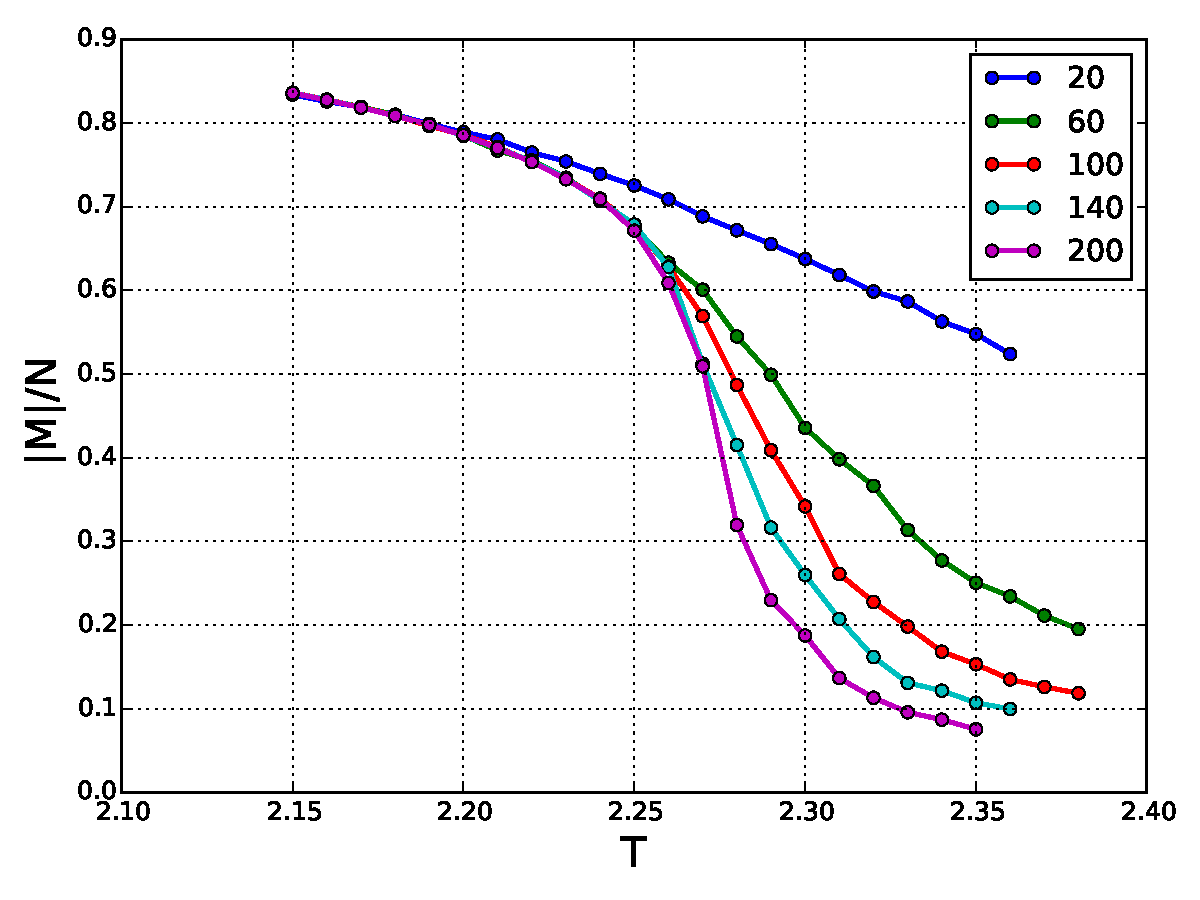
\includegraphics[width=\linewidth]{result/bilder/Tc/m-Tc}
        \caption{}
    \end{subfigure}
    \begin{subfigure}{0.5\textwidth}
    	\centering
    	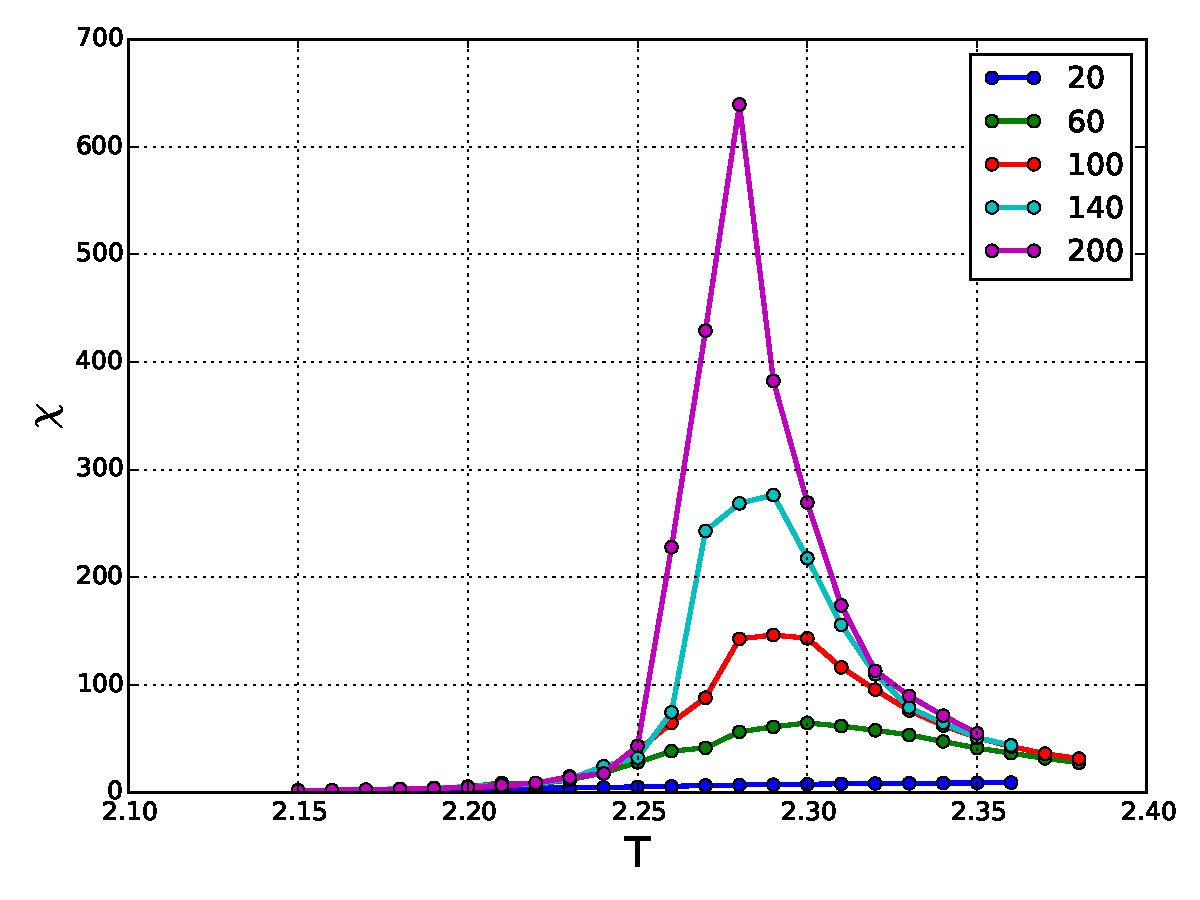
\includegraphics[width=\linewidth]{result/bilder/Tc/chi-Tc}
    	\caption{}
    \end{subfigure}%
    ~ 
    \begin{subfigure}{0.5\textwidth}
    	\centering
    	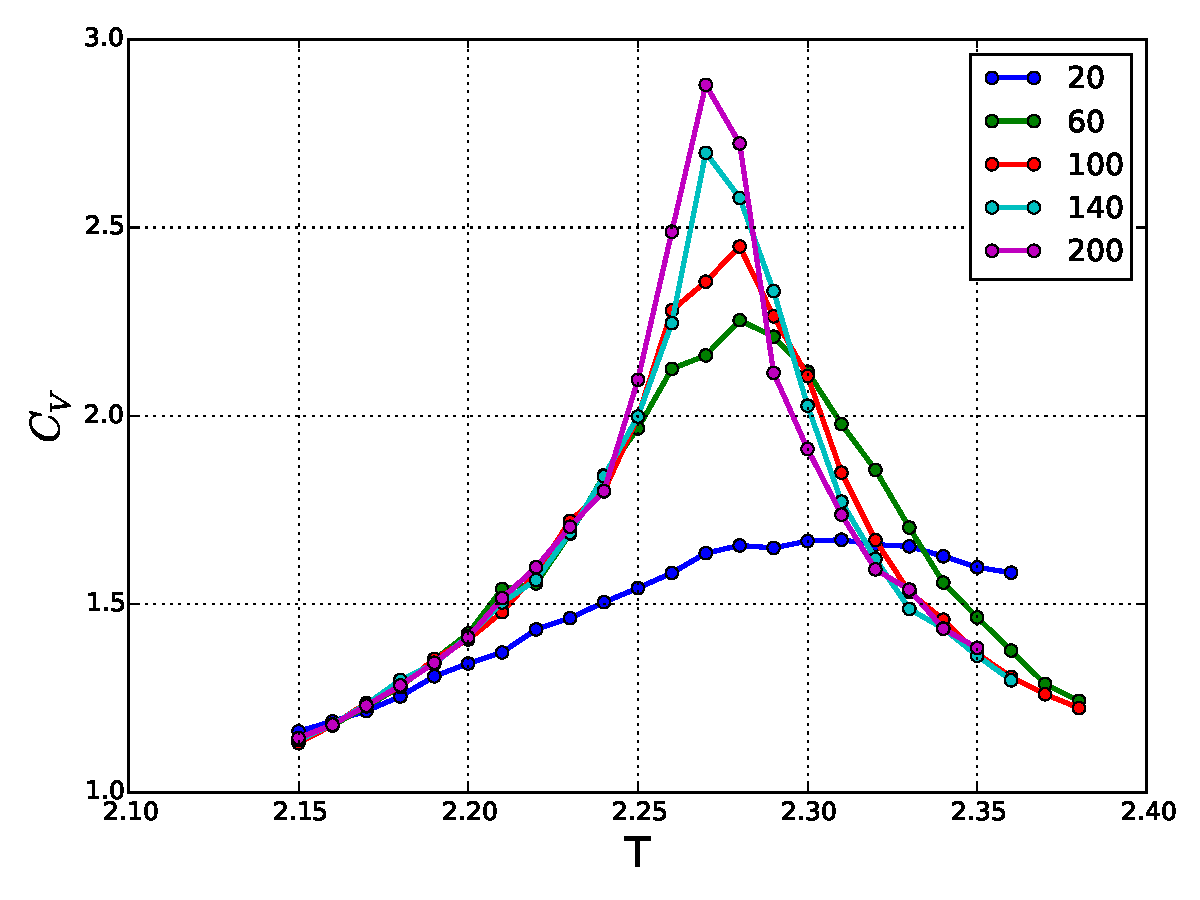
\includegraphics[width=\linewidth]{result/bilder/Tc/cv-Tc}
    	\caption{}
    \end{subfigure}
    \caption{Figures show the results for different temperatures $T$ plottet against energy(a), magnetisation(b), magnetic susceptibility(c) and heat capacity(d)}
    \label{fig:tc-chi-cv}
\end{figure}

The trends for the heat capacity shows a peak position. This should in theory correspond to the critical temperature. From the data it is clear that more data points are required to get a better result. Comparing the critical temperature to the magnetization gives a dip in magnetization close to the critical temperature. If the plots had been extended more two visible magnetization linear trends should be visible. One on each side of the phase transition. 










\pagebreak
\subsubsection{Critical temperature}
In the theory section a formula for the critical temperature was given. 

\begin{align*}
     &T_C (L) - T_C (L=\infty) = a L^{\frac{-1}{v}}
\end{align*}

 \begin{align*}
     &T_C (L_i) - T_C (L_j) = a 
     \left(
     L_i^{\frac{-1}{v}}-L_j^{\frac{-1}{v}}
     \right)
     \\
     &a = 
     \frac{T_C (L_i) - T_C (L_j)} 
     {
     L_i^{\frac{-1}{v}}-L_j^{\frac{-1}{v}}
     }
 \end{align*}
Applying this formula to the $L_i$ and $L_j$ plotted above gives a change in the variable $a$. The phase transistions are taken from the plots above. The cange in the variable $a$ will also be affected by ones choise of critical temperature. In this case the critical temperatures would be better if one had included more data points in the plot.

\begin{center}
\label{tab:extracting a}
\captionof{table}{The table shows how a differ for different $L_i$ and $L_j$  one uses.}
\begin{tabularx}{\textwidth}{|c| X c| X c| X c| X l|}
    \hline 
        $L_i$ && $L_j$ && $T_{C_i}$ && $T_{C_j}$ && a\\ 
    \hline
        60      &&      100     &&  2.30  &&  2.29  && 0.00025 \\
        60      &&      140     &&  2.30  &&  2.28  && 0.00025 \\
        60      &&      200     &&  2.30  &&  2.27  && 0.0002142 \\
        100     &&      140     &&  2.29  &&  2.28  && 0.00025 \\
        100     &&      200     &&  2.29  &&  2.27  && 0.0002 \\
        140     &&      200     &&  2.28  &&  2.27  && 0.0001666 \\
    \hline
\end{tabularx}
\end{center}

To get a common $T_C(\infty)$ the average of the different $a$'s are found. This is then plugged into the formula for $T_C(\infty)$. The results of $T_C(\infty)$ with the average $a$ is given in the table below:

\begin{center}
\label{tab:t-c}
\captionof{table}{Table giving $T_C(\infty)$ when the average of the variable $a$ is used.}
\begin{tabularx}{\textwidth}{|c| X c| X c| X |c| }
    \hline 
        $L_i$ && $T_C(L_i)$ && $T_C(\infty)$ \\ 
    \hline
        60      &&  2.30  && 2.2999\\
        100     &&  2.29  && 2.2899\\
        140     &&  2.28  && 2.2799\\
        200     &&  2.27  && 2.2699\\
    \hline
\end{tabularx}
\end{center}

An alternative way of finding $T_C$ is possible by linear regression of a plot with the different finite $T_C$ values plotted against the inverse of $L$. The intersection point of this regression line with the y-axis would give $T_C$ for a infinite lattice.

